% ===========================================================================
%  OSEMa bin-laden -- OSEM suspension damping: zero, alpha, beta, delta
%
%  Build:   tectonic talk.tex
%
%  Speaker notes are written with \note{} on every slide but are NOT shown by
%  default. To present with notes on a second screen, uncomment the
%  \setbeameroption line below and rebuild; each page then becomes slide+notes.
%  For a notes-only handout use \setbeameroption{show only notes}.
%
%  House style: no em-dashes anywhere in this file. Ranges use en-dashes.
% ===========================================================================
\documentclass[aspectratio=169]{beamer}

% \setbeameroption{show notes on second screen=right}

\usepackage{booktabs}
\usepackage{array}
\usepackage{tikz}
\usepackage{pgfplots}
\pgfplotsset{compat=1.18}
\usetikzlibrary{positioning,arrows.meta,automata,calc,fit,shapes.geometric}

\pgfplotsset{
  every axis/.append style={
    tick label style={font=\scriptsize},
    label style={font=\scriptsize},
    legend style={font=\scriptsize},
    title style={font=\small},
  },
}

\tikzset{
  blk/.style={draw, rounded corners, align=center, font=\scriptsize,
              minimum height=0.8cm, inner sep=3pt},
  every state/.style={rectangle, rounded corners, draw, align=center,
                      font=\scriptsize, minimum width=2.4cm, minimum height=0.8cm,
                      inner sep=2pt},
  flow/.style={-{Stealth[length=2mm]}, thick},
}

% === the three parts of every defect slide =================================
\newcommand{\rawdata}{\textbf{The data.}}
\newcommand{\goeswrong}{\textbf{What goes wrong.}}
\newcommand{\thefix}{\textbf{The fix, and the number that moved.}}

\title{OSEMa bin-laden}
\subtitle{Four rungs of a suspended-optic damping loop: \texttt{zero}, \texttt{alpha}, \texttt{beta}, \texttt{delta}}
\date{7 August 2026}

\begin{document}

% ================================================================ 1
\begin{frame}
  \titlepage
  \begin{center}
    \scriptsize Eight OSEM shadow sensors, eight coils, one suspended mirror,\\
    and four kept rungs of the supervisor around them.
  \end{center}
\end{frame}
\note{Title slide. The name is the project's own pun on OSEM. One control law,
barely changed since the first four-channel build, wrapped in a supervisor that
grew over four kept rungs. More builds existed between them; they are in version
control, not on this slide.

Every number in this deck is measured and comes out of the repository. Where a
number is a simulator number rather than a hardware number, the slide says so.

Every defect gets the same three-part treatment: the raw data, what goes wrong,
and the number that moved when it was fixed.}

% ================================================================ PART I
\section{The plant and the loop}

% ================================================================ 2
\begin{frame}{What is on the bench}
  \centering
  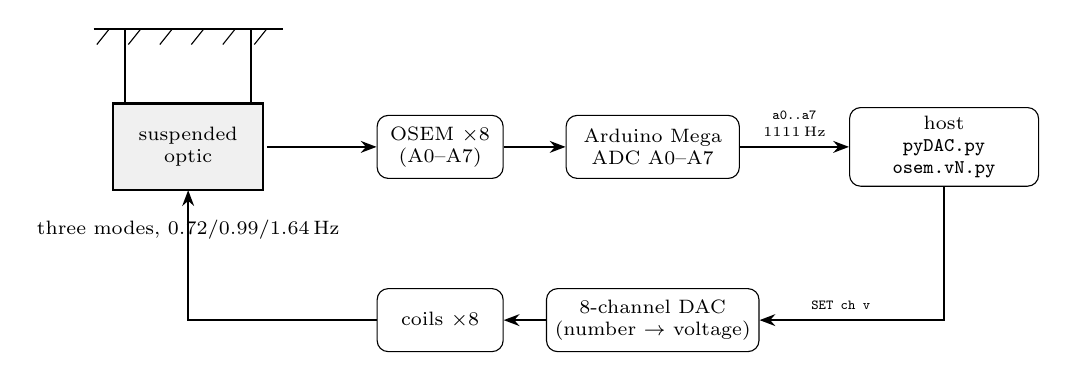
\begin{tikzpicture}[font=\scriptsize]
    \draw[thick] (-1.5,2.2) -- (0.9,2.2);
    \foreach \x in {-1.3,-0.9,...,0.8} \draw (\x,2.2) -- ++(-0.16,-0.2);
    \draw[thick] (-1.1,2.2) -- (-1.1,1.25);
    \draw[thick] (0.5,2.2) -- (0.5,1.25);
    \draw[thick, fill=gray!12] (-1.25,0.15) rectangle (0.65,1.25);
    \node[align=center] at (-0.3,0.7) {suspended\\optic};
    \node at (-0.3,-0.35) {three modes, $0.72 / 0.99 / 1.64$\,Hz};

    \node[blk, minimum width=1.6cm] (osem) at (2.9,0.7) {OSEM $\times$8\\(A0--A7)};
    \node[blk, minimum width=2.2cm] (adc)  at (5.6,0.7) {Arduino Mega\\ADC A0--A7};
    \node[blk, minimum width=2.4cm] (host) at (9.3,0.7) {host\\\texttt{pyDAC.py}\\\texttt{osem.vN.py}};
    \node[blk, minimum width=2.2cm] (dac)  at (5.6,-1.5) {8-channel DAC\\(number $\to$ voltage)};
    \node[blk, minimum width=1.6cm] (coil) at (2.9,-1.5) {coils $\times$8};

    \draw[flow] (0.7,0.7) -- (osem);
    \draw[flow] (osem) -- (adc);
    \draw[flow] (adc) -- node[above, align=center, font=\tiny]
      {\texttt{a0..a7}\\1111\,Hz} (host);
    \draw[flow] (host) |- node[pos=0.78, above, font=\tiny] {\texttt{SET ch v}} (dac);
    \draw[flow] (dac) -- (coil);
    \draw[flow] (coil.west) -| (-0.3,0.15);
  \end{tikzpicture}

  \vspace{2mm}
  \begin{minipage}{0.9\textwidth}\centering
  {\scriptsize Sensor $i$ $\to$ pin \texttt{A}$i$ $\to$
   \texttt{DAC\_CHANNELS} $=$ \texttt{[1,3,5,7,0,2,4,6]}.\\
   All eight OSEMs and all eight coils are connected. \\
   \textbf{Four} of them, a0--a3, carry usable in-band signal and
   their four coils push back.}
  \end{minipage}
\end{frame}
\note{One suspended mirror, eight OSEM shadow sensors, eight coils, and a host
closing the loop over a serial link.

The coil map is the thing to flag. Sensor i drives the coil at DAC_CHANNELS of i,
and that map is not the identity. Neither the simulator nor the interlocks can
catch a wrong map, because the simulator round-trips its held-voltage dictionary
through whatever map the controller declares. Only the bench catches that.}

% ================================================================ 3
\begin{frame}{The OSEM: a shadow sensor}
  \centering
  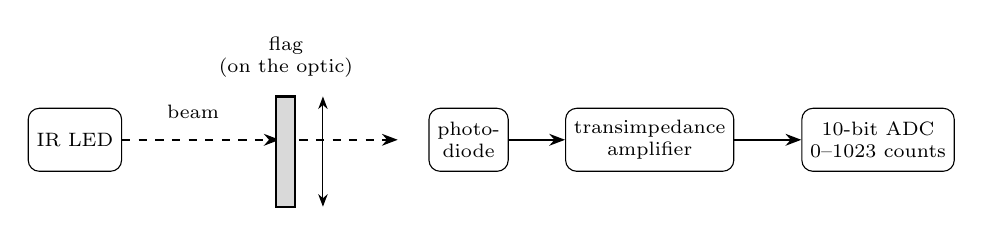
\begin{tikzpicture}
    \node[blk] (led) at (0,0) {IR LED};
    \draw[flow, dashed] (led) -- (2.6,0);
    \node[font=\scriptsize] at (1.5,0.35) {beam};
    \draw[thick, fill=gray!30] (2.55,-0.85) rectangle (2.8,0.55);
    \node[font=\scriptsize, align=center] at (2.68,1.05) {flag\\(on the optic)};
    \draw[{Stealth[length=1.6mm]}-{Stealth[length=1.6mm]}] (3.15,-0.85) -- (3.15,0.55);
    \draw[flow, dashed] (2.85,0) -- (4.1,0);
    \node[blk] (pd) at (5.0,0) {photo-\\diode};
    \node[blk] (tia) at (7.3,0) {transimpedance\\amplifier};
    \node[blk] (adc) at (10.2,0) {10-bit ADC\\0--1023 counts};
    \draw[flow] (pd) -- (tia);
    \draw[flow] (tia) -- (adc);
  \end{tikzpicture}

  \vspace{4mm}
  \footnotesize
  \begin{itemize}\setlength{\itemsep}{4pt}
    \item \textbf{An analogue-to-digital converter turns that voltage into a
          whole number, 0 to 1023 ``counts''.} Its two ends are the
          \emph{rails}: past them the number cannot go further, whatever the
          mirror does.
    \item \textbf{At a rail the sensor is outside its linear region}, so
          anything derived from it is wrong until the flag comes back.
  \end{itemize}
\end{frame}
\note{An infrared LED shining across a gap onto a photodiode, with a flag on the
optic partly blocking the beam. Move the optic, the shadow moves, the
photocurrent changes.

The first bullet is the one that dominates the whole project: the sensor is
linear only in partial shadow, so a channel that reaches a rail stops reporting
motion at all.

The two voltage scales are worth pausing on because conflating them is an easy
mistake to make when reading the code: 4.907 millivolts per count on the sensing
side, and a DAC that can reach 2.5 volts but is deliberately restricted to a
half-volt window on the actuation side.}

% ================================================================ 3b
\begin{frame}{How the damping was measured, and why it is a bound}
  \scriptsize
  \begin{columns}[T]
    \begin{column}{0.52\textwidth}
      \textbf{The normal way.} Kick the pendulum, remove all drive, watch the
      swing die away, fit the decay. One kick, one curve, and $Q$ follows.

      \vspace{1.5mm}
      \textbf{Two measured reasons that was impossible here.}
      \begin{itemize}\setlength{\itemsep}{1pt}
        \item \textbf{Too slow.} $\tau > 138$\,s needs five to ten minutes of
              undisturbed decay. Ambient building motion re-excites the mirror
              long before that.
        \item \textbf{A big enough kick saturates the sensor.} ch0 rests at
              $\sim$590 counts, so $\sim$430 counts of swing before it hits an
              end: only \textbf{7$\times$} the 62-count ambient, where fitting a
              decay wants \textbf{10$\times$}. The large-amplitude part, with
              the best signal, is the unusable part.
      \end{itemize}

      \vspace{1.5mm}
      \textbf{What was done instead.} A \textbf{320\,s recording with the loop
      off}, coils parked, \textbf{no kick}: 355\,797 samples, coils written 8
      times in the whole record, \textbf{nothing reaching a sensor end}.
    \end{column}
    \begin{column}{0.46\textwidth}
      \centering
      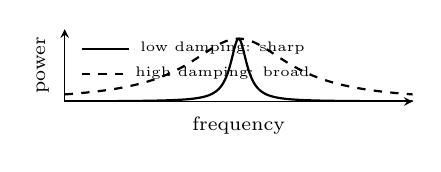
\begin{tikzpicture}
        \begin{axis}[width=6.0cm, height=2.5cm,
                     xlabel={frequency}, ylabel={power},
                     xmin=0.93, xmax=1.07, ymin=0, ymax=1.15,
                     axis lines=left, xtick=\empty, ytick=\empty,
                     legend style={at={(0.02,0.98)}, anchor=north west,
                                   draw=none, fill=none, font=\tiny}]
          \addplot[thick, domain=0.93:1.07, samples=400]
            {1/(1+((x-1)/0.004)^2)};
          \addlegendentry{low damping: sharp}
          \addplot[dashed, thick, domain=0.93:1.07, samples=300]
            {1/(1+((x-1)/0.025)^2)};
          \addlegendentry{high damping: broad}
        \end{axis}
      \end{tikzpicture}

      \raggedright
      \textbf{Why that still gives the damping.} Shaken by broadband noise, a
      resonance makes a peak, and the \textbf{width} of the peak is set by the
      damping: $\text{width} = f_0 / Q$. Measure the \emph{sharpness of the
      peak}, not the decay of a swing.

      \vspace{1.5mm}
      \textbf{Why it is a bound.} 276\,s of usable record resolves
      $1/276 = \mathbf{0.0036}$\,\textbf{Hz}. A mode at 0.7155\,Hz with
      $Q = 433$ is only $\mathbf{0.0017}$\,\textbf{Hz} wide, narrower than that.
      Measured width \textbf{0.00566}\,Hz against a resolution floor of
      \textbf{0.00543}.

      \vspace{1mm}
      ``At least as sharp as I can resolve'' bounds $Q$ from below and cannot
      give a value. \alert{\textbf{A longer quiet recording fixes that; a bigger kick
      does not.}}
    \end{column}
  \end{columns}

  \vspace{1.5mm}
  {\scriptsize \textbf{A caution.} An earlier attempt fitted decay curves from
  kicks during normal runs and got $Q = 20$--$22$, excluded at
  \textbf{21.7$\sigma$}: in all \textbf{73} windows the other three channels
  were still damping. It measured the control loop and reported it as the
  pendulum.}
\end{frame}
\note{The deck quotes Q greater than 433 and tau greater than 138 seconds, so it
owes you an account of where those came from. The file names in the repository
say ringdown, and this is not a classical ringdown, so I want to be careful.

Normally you kick a pendulum, take all the drive away, watch the swing die, and
fit the decay. One kick, one curve, and Q falls out of how fast it dies.

Two measured reasons that could not be done. First, it is too slow: with tau over
138 seconds you would need five to ten minutes of undisturbed decay, and ambient
building motion re-excites the mirror long before that. Second, a kick big enough
to measure saturates the sensor. Channel zero rests around 590 counts, so there
are about 430 counts of swing before it hits an end, which is only seven times
the ambient level, where fitting a decay properly wants a factor of ten. The
large-amplitude part of the swing, the part with the best signal, is exactly the
part that is unusable.

So instead: a 320 second recording with the control loop off and the coils
parked. No kick at all. The mirror simply moves under ambient excitation, and
nothing reaches a sensor end.

That still gives you the damping, and the picture is the reason. Shake a
resonance with broadband noise and it makes a peak in the spectrum. The width of
that peak is set by the damping: width equals f-nought over Q. Low damping means
a sharp peak. So you measure the sharpness of the peak instead of the decay of a
swing.

And that is also why the answer is a bound rather than a number. 276 seconds of
usable record resolves 0.0036 hertz. A mode at 0.7155 hertz with Q of 433 is
0.0017 hertz wide, narrower than the resolution. The measured width is 0.00566
against a resolution floor of 0.00543. So the honest statement is that the peak
is at least as sharp as I can resolve, which bounds Q from below and cannot
produce a value. A longer quiet recording turns it into a number. A bigger kick
does not.

The caution at the bottom is the trap. An earlier attempt did fit decay curves,
taken from kicks during normal runs, and got Q of twenty to twenty-two. That is
excluded at 21.7 sigma, because in all seventy-three of those windows the other
three channels were still actively damping. It measured the control loop and
reported it as the pendulum. In a ringdown you have to be certain nothing else is
removing energy.}

% ================================================================ 4
\begin{frame}{The plant: three resonances, and a bound on the damping}
  \begin{columns}[T]
    \begin{column}{0.47\textwidth}
      \footnotesize
      A suspended optic is a damped harmonic oscillator. For one sensed
      coordinate $x(t)$, mass $m$, force $F(t)$, and mode $m$:
      \[ \ddot{x} + \frac{\omega_m}{Q_m}\,\dot{x} + \omega_m^2 x = \frac{F(t)}{m} \]
      \vspace{-3mm}

      Amplitude decays as $e^{-\gamma_m t}$, so
      \[ \gamma_m = \frac{\omega_m}{2 Q_m}, \qquad \tau_m \equiv 1/\gamma_m. \]

      \vspace{2mm}
      \textbf{Resonances}, 320\,s ringdown, coils at bias:
      \[ f_A, f_B, f_C = 0.7155,\ 0.9949,\ 1.6396\ \mathrm{Hz} \]
      \vspace{-4mm}
      \begin{center}each $\pm 0.0001$\,Hz\end{center}
    \end{column}
    \begin{column}{0.51\textwidth}
      \footnotesize\raggedright
      $\gamma_m$ across channels, in s$^{-1}$:

      \vspace{1mm}
      \centering
      {\scriptsize
      \begin{tabular}{@{}lccc@{}}
        \toprule
        & ch & median & range \\
        \midrule
        A & 4 & 0.0483 & $0.0107$--$0.1388$ \\
        B & 5 & 0.0082 & $0.0005$--$0.0579$ \\
        C & 4 & 0.0094 & $0.0061$--$0.0530$ \\
        \bottomrule
      \end{tabular}}

      \vspace{1mm}
      \raggedright
      Mode A spans a \textbf{factor of 13} across four channels watching one
      rigid body, which a rigid body cannot do.
      \alert{\textbf{Do not quote a per-mode $\gamma$ as measured.}}

      \vspace{1.5mm}
      \textbf{What is established is \emph{aggregate}}, from a 12\,s
      autocorrelation exclusion test over all channels and the in-band signal as
      a whole. The fitted
      $\gamma_{\mathrm{agg}} = +0.00004 \pm 0.00719$\,s$^{-1}$ is consistent with
      zero:
      \[ Q > 433\ (1\sigma) \;\Rightarrow\; \tau > 138\,\mathrm{s} \]
      \vspace{-2mm}
      \alert{\textbf{One bound over all three modes, not three measurements.}}

      \vspace{1.5mm}
      {\scriptsize Closed loop the same kick settles in \textbf{2.9--4.7\,s}.}
    \end{column}
  \end{columns}
\end{frame}
\note{The plant, from a 320 second quiet ringdown with the coils held at bias.

Start with the notation, because it is the thing a physicist will check. Gamma
is per mode: gamma-m equals omega-m over two Q-m. Three resonances means three
gammas, and the slide should not pretend otherwise.

The resonances themselves are solid: 0.7155, 0.9949 and 1.6396 hertz, each to a
tenth of a millihertz.

The per-mode decay rates are not. Fit gamma per mode per channel and mode A comes
out anywhere from 0.0107 to 0.1388 per second, a factor of thirteen, across four
channels watching one rigid body. A rigid body does not have four different decay
rates for the same mode. Those fits are noise-dominated and I am not going to
quote one as a measurement.

What is established is an aggregate. A twelve second autocorrelation exclusion
test, run over all channels and the in-band signal as a whole, asks whether a
claimed Q is compatible with the observed decay of correlation. The aggregate
fitted rate is four times ten to the minus five, plus or minus 0.0072 per second,
consistent with zero. At one sigma that gives tau greater than 138 seconds and Q
greater than 433. One bound covering all three modes, not three measurements.

For scale: closed loop the same kick settles in three to five seconds. And a
sixteen second figure still carried in the simulator assumes Q of fifty, which
this test excludes at 8.7 sigma.}

% ================================================================ 5
\begin{frame}{Cold damping: the process variable is \emph{velocity}}
  \begin{align*}
    \mathrm{bp}(t) &= \mathrm{LP}_{3\,\mathrm{Hz}}\big[\,\mathrm{HP}_{0.4\,\mathrm{Hz}}[A(t)]\,\big] \\[2pt]
    \hat{v}(t) &= \mathrm{LP}_{5\,\mathrm{Hz}}\!\left[\frac{\mathrm{bp}(t)-\mathrm{bp}(t-\Delta t)}{\Delta t}\right] \\[2pt]
    u(t) &= -K_p(t)\cdot \hat{v}(t)
  \end{align*}
  \vspace{-2mm}
  \begin{center}
  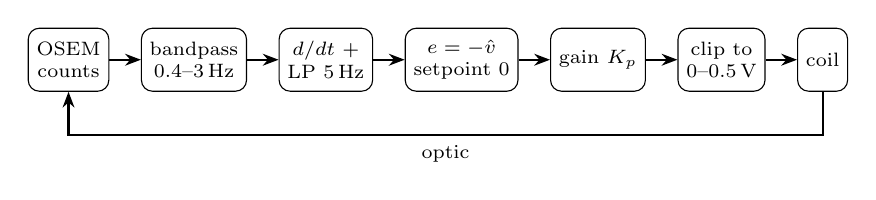
\begin{tikzpicture}[node distance=4mm]
    \node[blk] (osem) {OSEM\\counts};
    \node[blk, right=of osem] (bp) {bandpass\\0.4--3\,Hz};
    \node[blk, right=of bp] (dv) {$d/dt$ +\\LP 5\,Hz};
    \node[blk, right=of dv] (err) {$e = -\hat{v}$\\setpoint 0};
    \node[blk, right=of err] (pid) {gain $K_p$};
    \node[blk, right=of pid] (dac) {clip to\\0--0.5\,V};
    \node[blk, right=of dac] (coil) {coil};
    \foreach \a/\b in {osem/bp, bp/dv, dv/err, err/pid, pid/dac, dac/coil}
      \draw[flow] (\a) -- (\b);
    \draw[flow] (coil.south) -- ++(0,-0.55) -| node[pos=0.25, below, font=\scriptsize]
      {optic} (osem.south);
  \end{tikzpicture}
  \end{center}
  \vspace{1mm}
  {\footnotesize \textbf{The bandpass keeps only the part of the signal between
  0.4 and 3\,Hz}, discarding slow drift below and fast noise above. All three
  measured resonances sit inside that window. The target is a constant zero, so
  the error is just minus the speed: the loop never asks where the mirror
  \emph{is}, only that it stop \emph{moving}.}
\end{frame}
\note{The critical thing, and what makes textbook intuition misleading here, is
that the process variable is velocity and the setpoint is a constant zero. So the
error is simply minus the velocity. The loop has no opinion about where the optic
sits; it only objects to it moving. That is cold damping: synthesising a viscous
drag the suspension deliberately does not have.

The bandpass matters. All three measured modes sit inside 0.4 to 3 hertz. A mode
outside that band would be filtered out of the very signal the loop closes on.}

% ================================================================ 6
\begin{frame}{Three gains: P is a damper, I is a spring, D is a mass}
  \centering
  {\footnotesize A \textbf{PID controller} combines three responses to an error:
  one proportional to it, one to its running total, one to its rate of change.
  Here the ``error'' is the mirror's speed, which shifts what each term means.}

  \vspace{1mm}
  With $e = -\hat{v}$ and $\hat{v} \approx \dot{x}$, the velocity of the sensed
  coordinate $x$:
  \[
    \underbrace{K_p\,e = -K_p\,\dot{x}}_{\text{force} \propto \text{velocity}}
    \qquad
    \underbrace{K_i\!\int\! e\,dt = -K_i\,x}_{\text{force} \propto \text{displacement}}
    \qquad
    \underbrace{K_d\,\frac{de}{dt} = -K_d\,\ddot{x}}_{\text{force} \propto \text{acceleration}}
  \]
  \vspace{1mm}
  {\footnotesize
  \begin{tabular}{@{}llll@{}}
    \toprule
    term & acts on & physically & effect on the pole \\
    \midrule
    $K_p$ & velocity & \textbf{viscous damper} & \alert{\textbf{the only term that removes energy}} \\
    $K_i$ & displacement & added \textbf{spring} & moves the resonance; does not damp \\
    $K_d$ & acceleration & added (negative) \textbf{mass} & noisiest; differentiates twice \\
    \bottomrule
  \end{tabular}}

  \vspace{3mm}
  \begin{minipage}{0.9\textwidth}
  \footnotesize
  \textbf{Why add I and D at all?} $K_p$ sets the damping, but it leaves a steady
  offset it cannot remove and it reacts only to present error. $K_i$ takes out the
  offset; $K_d$ anticipates (and therefore useless for us)

  \end{minipage}
\end{frame}
\note{The one slide that will surprise anyone who knows ordinary PID.

Because the error is minus velocity, every term is shifted by one derivative from
what its name suggests. That is the whole content of the table, and it is why the
integrator is a spring rather than a drift-remover here.

The question the table leaves hanging is why add I and D at all. P sets the
damping but leaves a steady offset it cannot remove and reacts only to present
error. I takes out the offset, D anticipates. Neither dissipates, so amplitude
ratio is simply not the number either would move.
}

% ================================================================ 7
\begin{frame}{How hard to push: choosing the gain}
  \scriptsize
  \begin{columns}[T]
    \begin{column}{0.53\textwidth}
      \begin{enumerate}\setlength{\itemsep}{2.5pt}
        \item The controller measures \textbf{how fast the mirror is moving} and
              pushes against that motion. Push harder, it settles sooner.
        \item \textbf{The gain is the constant relating the two.} Speed arrives
              as volts per second of sensor signal, the push leaves as a voltage
              on the coil, so $K_p$ is in \textbf{volts per volt-per-second}.
        \item \alert{\textbf{It is negative because the push must oppose the motion.}} A
              positive value pushes the way the mirror is already going, feeding
              the motion instead of removing it.
        \item \textbf{Two ceilings stop it going up indefinitely.} Above about
              $0.040$ the loop was seen on an oscilloscope to go unstable. And
              the coil drive has a fixed $\pm 0.25$\,V window, past which the
              loop asks for more push than the hardware can give.
        \item \textbf{$0.035$ fits under both, and \emph{instability} binds}:
              the budget at $0.035$ is \textbf{0.2001\,V} of $0.250$\,V, so the
              hardware still has room when stability runs out.
      \end{enumerate}
    \end{column}
    \begin{column}{0.45\textwidth}
      \centering
      {\scriptsize\setlength{\tabcolsep}{2.5pt}
      \begin{tabular}{@{}lrrrr|c@{}}
        \toprule
        & ch0 & ch1 & \textbf{ch2} & ch3 & ch4--7 \\
        \midrule
        $K_p$ & $-.035$ & $-.035$ & $\mathbf{+.035}$ & $-.035$ & $0$ \\
        $K_i$ & $-.0060$ & $-.0060$ & $\mathbf{+.0060}$ & $-.0060$ & $0$ \\
        $K_d$ & $-.00045$ & $-.00045$ & $\mathbf{+.00045}$ & $-.00045$ & $0$ \\
        \bottomrule
      \end{tabular}}

      \vspace{2mm}
      \raggedright
      \textbf{ch2 is positive, and that is correct.} Its sensor and coil are
      mounted the opposite way round, so there opposing the motion \emph{means}
      the opposite sign. It damps fastest of the four while running positive.

      \vspace{2mm}
      $K_i$ and $K_d$ take each channel's sign, because all three push the same
      coil. \textbf{ch4--ch7 sit at zero}: which way their coils push is not
      known, and a wrong sign would feed the motion.

      \vspace{1.5mm}
      {\scriptsize Only $|K_p| = 0.030$ was fixed by watching an oscilloscope:
      $6\times$ reduction, no clipping.}
    \end{column}
  \end{columns}
\end{frame}
\note{This is the slide to go slowly on, because everything later depends on it.

The controller measures how fast the mirror is moving and pushes against that
motion. Push harder, it settles sooner. The gain is just the constant relating
those two things, and because speed arrives as volts per second of sensor signal
and the push leaves as a voltage on a coil, the gain is in volts per
volt-per-second.

The sign is the part worth saying out loud. It is negative because the push has
to oppose the motion. Get the sign wrong and you are pushing the mirror the way
it is already going, which feeds the swing rather than removing it.

Then why not simply turn it up. Two separate ceilings. One is stability: above
about 0.040 the loop was watched on an oscilloscope going unstable. The other is
hardware: the coil drive has a fixed half-volt window and past a point the loop
asks for more than the electronics can deliver. 0.035 fits under both, and it is
the instability ceiling that binds, because the actuator budget at that gain comes
to 0.2001 volts of the 0.250 available.

Channel two is positive and it is not a typo. Its sensor and its coil are mounted
the opposite way round, so on that one channel opposing the motion means the
opposite sign. Three separate measurements agree, including that it damps fastest
of the four while running positive.

And channels four to seven sit at zero because nobody knows which way their coils
push. A guessed sign there would feed the motion.}

% ================================================================ 10
\begin{frame}{The gain is not one fixed number}
  \scriptsize
  \begin{columns}[T]
    \begin{column}{0.50\textwidth}
      \textbf{What a gain schedule is.} The gain changes with \emph{how far the
      mirror currently is from rest}. Two values are declared, a
      \textbf{steady} one for small motion and a \textbf{capture} one for large,
      and the controller blends between them.

      \vspace{1.5mm}
      \textbf{How ``far from rest'' is measured.} Once per run, gain forced to
      zero, the controller records the typical size of the sensor signal: the
      \textbf{baseline}, meaning this room tonight with nothing driving.
      Everything afterwards is a \textbf{ratio} to it, so $r = 1$ is ``as lively
      as when we were not pushing''.

      \vspace{1.5mm}
      \textbf{The blend.} Full capture above $r = 0.6$, tapering to steady by
      $r = 0.2$, rate-limited to $0.02$ per second so no gain change can itself
      jolt the mirror. That ramp is also the startup soft-start, 1.75\,s.

      \vspace{1.5mm}
      \textbf{In the shipping controller both values are $\pm 0.035$.} The
      blend therefore does nothing, and the rate limit and soft-start are its
      only live effects. \alert{\textbf{No reason for having two levels is recorded
      anywhere in the project.}}
    \end{column}
    \begin{column}{0.48\textwidth}
      \centering
      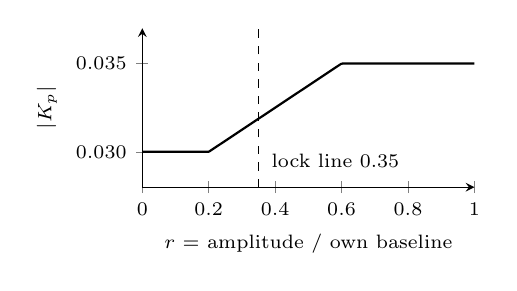
\begin{tikzpicture}
        \begin{axis}[width=5.8cm, height=3.6cm,
                     xlabel={$r$ = amplitude / own baseline},
                     ylabel={$|K_p|$}, scaled y ticks=false,
                     xmin=0, xmax=1.0, ymin=0.028, ymax=0.037,
                     axis lines=left, ytick={0.030,0.035},
                     yticklabels={$0.030$, $0.035$}]
          \addplot[thick, samples=200, domain=0:1]
            {0.030 + 0.005*max(0,min(1,(x-0.2)/0.4))};
          \draw[dashed] (axis cs:0.35,0.028) -- (axis cs:0.35,0.037);
          \node[font=\scriptsize, anchor=west] at (axis cs:0.36,0.0295) {lock line 0.35};
        \end{axis}
      \end{tikzpicture}\\
      {\scriptsize The declared shape. Shown with two distinct levels; the
      shipping controller sets both to $0.035$.}

      \vspace{2mm}
      \raggedright
      \textbf{That one baseline does three jobs}, which is why so much later
      work is about how it is measured:
      \begin{itemize}\setlength{\itemsep}{1pt}
        \item the runaway breaker trips above $1.8 \times$ baseline
        \item the blend runs between $0.2\times$ and $0.6\times$
        \item \texttt{LOCKED} means below $0.35\times$, held 5\,s
      \end{itemize}
    \end{column}
  \end{columns}
\end{frame}
\note{Two ideas here, and neither is standard vocabulary, so take them slowly.

A gain schedule just means the gain is not one fixed number: it changes with how
far the mirror currently is from rest. Two values are declared, a steady one for
small motion and a stronger capture one for large motion, and the controller
blends between them.

That needs a yardstick for how far from rest, and the yardstick is the baseline.
Once per run, with the gain forced to zero, the controller records the typical
size of the sensor signal. That is this room on this night with nothing driving.
Everything afterwards is quoted as a ratio to it, so a ratio of one means as
lively as when we were not pushing.

The blend is full capture above 0.6 of baseline, tapering to steady by 0.2, and
every change is rate-limited to 0.02 per second so that the gain change cannot
itself jolt the mirror. That same ramp is the startup soft-start.

Now the honest part. In the shipping controller both values are the same, plus or
minus 0.035. So the blend does nothing at all, and the rate limit and soft-start
are the only live effects of the schedule. And I could not find any recorded
justification for having two levels in the first place, in the source, in the
version notes or anywhere else. I am flagging that rather than inventing a
motivation for it.

The right-hand list is why the baseline matters out of proportion to its size.
One number, measured once in one window, sets the fault threshold, the gain blend
and the definition of success.}

% ================================================================ 12
\begin{frame}{The wire is the bottleneck, and the loop rate falls with coil count}
  \begin{columns}[T]
    \begin{column}{0.49\textwidth}
      \centering
      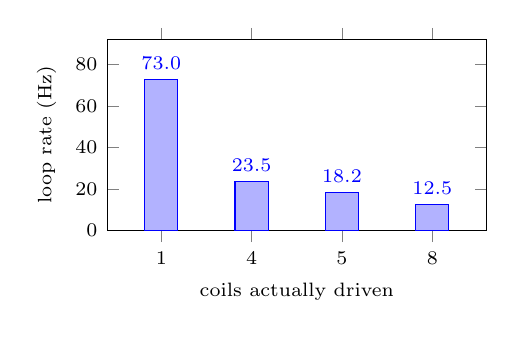
\begin{tikzpicture}
        \begin{axis}[width=6.4cm, height=4.0cm, ybar, bar width=12pt,
                     symbolic x coords={1, 4, 5, 8},
                     xtick=data, ymin=0, ymax=92,
                     ylabel={loop rate (Hz)},
                     xlabel={coils actually driven},
                     nodes near coords={\pgfmathprintnumber[fixed,zerofill,precision=1]{\pgfplotspointmeta}},
                     every node near coord/.append style={font=\scriptsize},
                     enlarge x limits=0.20]
          \addplot coordinates {(1,73.0) (4,23.5) (5,18.2) (8,12.5)};
        \end{axis}
      \end{tikzpicture}\\
      {\scriptsize Median \texttt{DAMPING}-row spacing over 20 bench logs:
      13.7 / 42.6 / 55.0 / 79.9\,ms.}

      \vspace{1mm}
      {\scriptsize \textbf{Same run, both states:} \textbf{357.1\,Hz} while
      \texttt{CALIBRATING} with no coil writes against \textbf{18.2\,Hz} while
      \texttt{DAMPING} on 5 coils. \textbf{A factor of 19.6}, with no
      between-run variation to argue about.}
    \end{column}
    \begin{column}{0.49\textwidth}
      \footnotesize\raggedright
      \texttt{set\_voltage} blocks reading up to 50 stream lines waiting for its
      \texttt{OK}. \textbf{Every coil write costs a serial round trip}, so the
      loop rate is set by how many coils are driven, not by the control law.

      \vspace{2mm}
      \textbf{Exactly one} threshold was counted in \emph{samples} rather than
      seconds, so its meaning moved with the coil count:

      \vspace{1mm}
      \centering
      {\scriptsize
      \begin{tabular}{@{}lrrrr@{}}
        \toprule
        \multicolumn{5}{@{}l}{\texttt{MAX\_CONSECUTIVE\_SATURATED = 30}} \\
        \midrule
        coils & 1 & 4 & 5 & 8 \\
        means & 0.41\,s & \textbf{1.28\,s} & 1.65\,s & \textbf{2.40\,s} \\
        \bottomrule
      \end{tabular}}

      \vspace{2mm}
      \raggedright
      \alert{Less sensitive exactly as the rig got harder to control.}

      \vspace{1.5mm}
      And it costs phase. Margin at 3.75\,Hz: \textbf{73.5$^\circ$} on
      4 coils, \textbf{45.5$^\circ$} on 8, \textbf{105.0$^\circ$} once the ack
      wait goes. \textbf{Every gain in the rig was fixed on a 4-coil loop.}
    \end{column}
  \end{columns}
\end{frame}
\note{A measurement that changed how we read every timing number in the project.

The control loop rate depends on how many coils are being driven: 73 hertz with
one coil, 23.5 with four, 18.2 with five and 12.5 with eight. The cause is the
transport: every coil write blocks reading up to fifty stream lines waiting for
its acknowledgement.

The cleanest version of that number comes from a single run rather than from
comparing runs. 357.1 hertz while calibrating, where no coil is written, and 18.2
while damping five coils. Same optic, same minute, a factor of 19.6 that is purely
the transport.

That also fixes what the gains mean. The phase budget makes it concrete: 73.5
degrees of margin at 3.75 hertz on four coils, 45.5 on eight, and 105.0 once the
ack wait is removed. Every gain in the rig was fixed on the four-coil loop, so
carrying those gains onto eight coils halves the margin they were chosen with.

And exactly one threshold in the codebase was counted in samples rather than
seconds. Thirty consecutive saturated samples is 0.41 seconds on one coil and
2.40 on eight, so the saturation interlock got less sensitive precisely as the rig
got harder to control.}


% ================================================================ 14
\begin{frame}{The supervisor: three states}
  \centering
  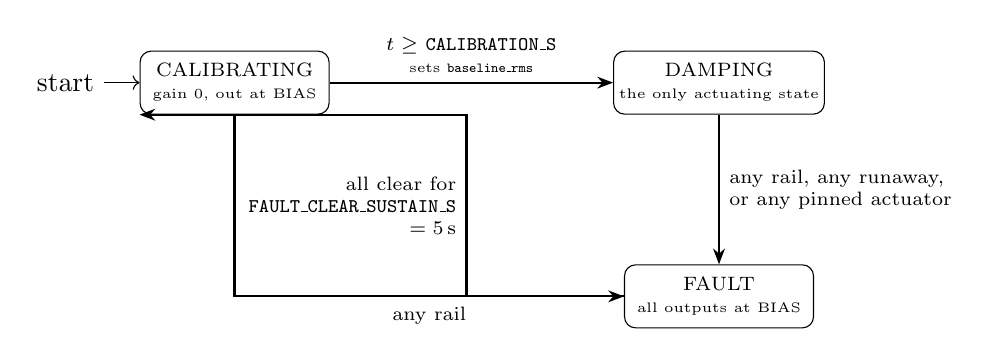
\begin{tikzpicture}[node distance=3.2cm and 3.6cm]
    \node[state, initial, initial text={start}] (C) {CALIBRATING\\{\tiny gain 0, out at BIAS}};
    \node[state, right=of C] (D) {DAMPING\\{\tiny the only actuating state}};
    \node[state, below=1.9cm of D] (F) {FAULT\\{\tiny all outputs at BIAS}};
    \draw[flow] (C) -- node[above, font=\scriptsize, align=center]
      {$t \geq$ \texttt{CALIBRATION\_S}\\{\tiny sets \texttt{baseline\_rms}}} (D);
    \draw[flow] (D) -- node[right, font=\scriptsize, align=left]
      {any rail, any runaway,\\or any pinned actuator} (F);
    \draw[flow] (C.south) |- node[pos=0.75, below, font=\scriptsize] {any rail} (F.west);
    \draw[flow] (F.west) -- ++(-2.0,0) |- node[pos=0.25, left, font=\scriptsize, align=right]
      {all clear for\\\texttt{FAULT\_CLEAR\_SUSTAIN\_S}\\$= 5$\,s} (C.south west);
  \end{tikzpicture}

  \vspace{2mm}
  {\footnotesize
  \textbf{No transition out of \texttt{DAMPING} except into \texttt{FAULT}}, and
  no terminal state. \texttt{Ctrl+C} leaves through a \texttt{finally} block that
  returns every DAC channel to bias.}

  \vspace{1mm}
  {\footnotesize What does \emph{not} run in \texttt{FAULT}: the gain
  schedule, the runaway check and the lock update. Any flag those set on the way
  in is therefore never recomputed while the fault is held.}
\end{frame}
\note{One string variable, three values. It gates actuation and is written to
every CSV row, and the simulator drives the shipping code through this same state
machine rather than reimplementing it.

Two structural points. There is no way out of DAMPING except into FAULT, and no
terminal state: Ctrl-C leaves through a finally block that returns every DAC
channel to bias.

And the box at the bottom is the first defect. The schedule update, the runaway
check and the lock update are all skipped in FAULT, so a flag set on the way in
is never recomputed.}

% ================================================================ PART II
\section{The ladder}

% ================================================================ 15
\begin{frame}{\texttt{zero}: the original}
  \begin{columns}[T]
    \begin{column}{0.55\textwidth}
      \footnotesize
      \texttt{ENABLE\_CHANNEL = [True, False, False, False]}\\
      P-only: $u = -K\cdot v$, \texttt{KI\_GAIN} $=$ \texttt{KD\_GAIN} $= 0$.

      \vspace{2mm}
      \textbf{What \texttt{zero} got right, and every version since inherits:}
      \begin{enumerate}\setlength{\itemsep}{1pt}
        \item Runs continuously, not as fixed-duration sweep steps.
        \item Measures its \emph{own} baseline every restart.
        \item A rail interlock on \emph{raw counts}, separate from the RMS
              breaker. A blind OSEM flatlines, which an RMS-only check reads as
              perfect stability.
        \item Auto-recovery out of \texttt{FAULT}.
        \item A lock detector that prints a real number.
        \item Streaming CSV, flushed periodically, survives an unclean kill.
        \item Gain scheduling with a slew-limited ramp.
      \end{enumerate}
    \end{column}
    \begin{column}{0.43\textwidth}
      \centering
      {\scriptsize
      \begin{tabular}{@{}lr@{}}
        \toprule
        \multicolumn{2}{@{}l}{\textbf{\texttt{zero}, through \texttt{harness.py}}} \\
        \midrule
        ch0 amplitude ratio & 0.188 \\
        time to lock        & 12.1\,s \\
        suite (when present)& 18/18 \\
        \midrule
        undriven ch1/2/3    & 0.333 / 0.316 / 0.253 \\
        \bottomrule
      \end{tabular}}

      \vspace{3mm}
      \footnotesize
      \raggedright
      \textbf{Three defects shipped with it} and survived into the next two
      builds: \texttt{saturation-latch}, \texttt{rail-threshold},
      \texttt{runaway-baseline}. All three are fixed in \texttt{alpha}.

      \vspace{2mm}
      Plus a fourth nobody found until \texttt{beta}, and a fifth until \texttt{delta}.
    \end{column}
  \end{columns}
\end{frame}
\note{the zero build is the 2026-07-15 bench configuration: channel zero only, pure velocity
feedback, I and D zeroed. It is the only entry in the ladder confirmed against a
scope.

The left column is the design that survived. Seven things no later version
changed.

The rail interlock deserves a moment. A fully occluded OSEM pins the ADC at
zero, and the bandpassed signal then flatlines near zero, which looks like
perfect stability to an RMS check at the exact moment the sensor has gone blind.
So rail state is checked on raw counts, not on scaled voltage.

It shipped three defects, a fourth nobody found until beta, and a fifth until delta.}

% ================================================================ 19
\begin{frame}{Defect 1: \texttt{saturation-latch}}
  \begin{columns}[T]
    \begin{column}{0.50\textwidth}
      \footnotesize
      \rawdata\ An early four-channel run, ch0 output against the
      \texttt{VMAX} $= 0.5$\,V rail:

      \vspace{1mm}
      \centering
      {\scriptsize\ttfamily
      \begin{tabular}{@{}l l@{}}
        \toprule
        u (V) & sat\_streak \\
        \midrule
        0.4987 & 0 \\
        0.5000 & 1 \\
        $\;\;\vdots$ & $\;\;\vdots$ \\
        0.5000 & 30 \quad\rm trip \\
        0.5000 & 31 \\
        \bottomrule
      \end{tabular}}

      \vspace{1.5mm}
      \raggedright
      Without the integral term the streak reached \textbf{28} and never
      tripped. Switching it on added the three samples that crossed
      \textbf{30}.

      \vspace{1.5mm}
      \textbf{The smoking gun.} Across \textbf{16{,}966} \texttt{FAULT} samples
      \alert{the run logged \textbf{one} distinct ratio value: \textbf{3.6803}.}
    \end{column}
    \begin{column}{0.47\textwidth}
      \footnotesize
      \goeswrong\ \texttt{saturated\_flag} is recomputed only inside
      \texttt{check\_runaway()}, which does not run in \texttt{FAULT}.

      \vspace{1mm}
      \centering
      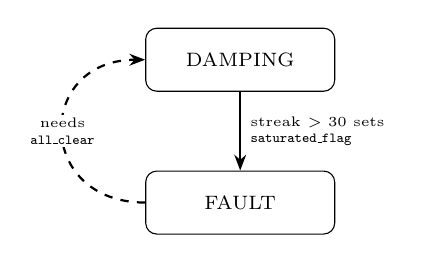
\begin{tikzpicture}[node distance=1.2cm]
        \node[state] (D) {DAMPING};
        \node[state, below=1.0cm of D] (F) {FAULT};
        \draw[flow] (D) -- node[right, font=\tiny, align=left]
          {streak $>30$ sets\\\texttt{saturated\_flag}} (F);
        \draw[flow, dashed] (F.west) .. controls +(-1.4,0) and +(-1.4,0) ..
          node[pos=0.5, font=\tiny, align=center, fill=white, inner sep=1pt]
          {needs\\\texttt{all\_clear}} (D.west);
      \end{tikzpicture}\\
      {\scriptsize The flag can never clear: permanent fault.}

      \vspace{1.5mm}
      \raggedright
      A \emph{runaway} trip recovered fine. \textbf{Only saturation deadlocked.}

      \vspace{1.5mm}
      \thefix\ \texttt{alpha} maintains the flag in \texttt{actuate()}, so it refreshes every
      sample in every state. In \texttt{FAULT} the output is at bias, so it
      clears itself.

      \vspace{1mm}
      That run latched $\sim$50\,s. \textbf{With the fix, same bench: 0 pinned
      samples, 0.00\% ADC clipped, no fault.}
    \end{column}
  \end{columns}
\end{frame}
\note{The first of the three original defects, and the only one reproduced on
hardware.

The data column is the mechanism. The saturation interlock counts consecutive
samples with the output pinned at a rail. Without the integral term the streak
reached 28 against a threshold of 30 and never tripped. Switching the integral
term on contributed the extra push and the streak reached 31. Three samples decided whether the run recovered.

The failure is not the trip, it is what happens next. the zero build recomputes the
saturated flag only inside check-runaway, and check-runaway does not run in the
FAULT state. So a saturation trip sets the flag, enters FAULT, and nothing can
ever clear it: permanent fault requiring a manual restart, in a module that
advertises auto-recovery. A runaway trip recovered fine because it never set that
flag. Only saturation deadlocked.

The evidence that it was the stale flag rather than a live condition is the
smoking gun on the slide: across 16,966 FAULT samples there is exactly one
distinct ratio value, 3.6803. If anything were being recomputed there would be
sixteen thousand different values.

The fix is to maintain the flag in actuate, where the output is actually known,
so it refreshes every sample in every state. In FAULT the output is held at bias,
so it clears on its own. alpha on the same bench had zero pinned samples and no
fault at all.}

% ================================================================ 20
\begin{frame}{Defect 2: \texttt{rail-threshold}, an interlock at the noise floor}
  \begin{columns}[T]
    \begin{column}{0.50\textwidth}
      \footnotesize
      \rawdata\ \texttt{zero}'s test: raw counts below \texttt{RAIL\_LOW\_COUNTS} $= 3$ of
      1023, i.e. \textbf{14.7\,mV}, for \textbf{250 consecutive} samples.

      \vspace{1mm}
      A blind channel with $\sim$1 count of dark noise:

      \vspace{1mm}
      \centering
      {\scriptsize\ttfamily
      \begin{tabular}{@{}l@{\;}l@{}}
        \toprule
        counts & consecutive count \\
        \midrule
        0 1 2 0 1 & 5 \\
        0 2 1 3 0 & 10 \\
        4 & $\to$ 0 \\
        1 0 2 & 3 \\
        \bottomrule
      \end{tabular}}

      \vspace{2mm}
      \raggedright
      \textbf{One sample above 3 counts erases everything.} The channel is
      blind the whole time.

      \vspace{2mm}
      \textbf{On hardware:} a four-channel run logged \textbf{246} genuinely clipped ADC samples
      (2.19\% of the run) and \alert{\textbf{the rail flag never set once}}.
    \end{column}
    \begin{column}{0.47\textwidth}
      \footnotesize
      \goeswrong\ Above $\sim$1 count RMS of dark noise the interlock
      \textbf{stops arming}. A blind channel's bandpassed output flatlines, so
      its ratio goes to \emph{zero}: it reads as the \textbf{steadiest axis on
      the rack} while the loop declares itself locked on a dead sensor.

      \vspace{2mm}
      \thefix\ \texttt{alpha}: threshold 3 $\to$ \textbf{12 counts}, and the test becomes
      \textbf{80\% of a 0.5\,s window} instead of an unbroken run. Noise now
      \emph{dilutes} the evidence instead of erasing it.

      \vspace{1mm}
      \centering
      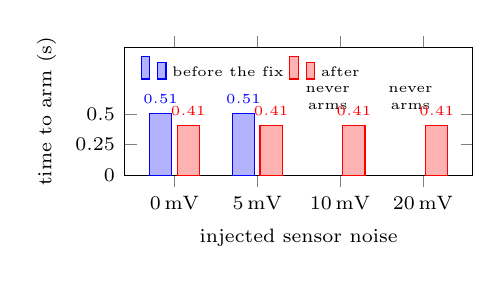
\begin{tikzpicture}
        \begin{axis}[width=6.0cm, height=3.2cm, ybar, bar width=8pt,
                     xtick={1,2,3,4},
                     xticklabels={0\,mV, 5\,mV, 10\,mV, 20\,mV},
                     xmin=0.4, xmax=4.6, ymin=0, ymax=1.05,
                     ytick={0,0.25,0.5},
                     ylabel={time to arm (s)},
                     xlabel={injected sensor noise},
                     legend style={at={(0.02,0.98)}, anchor=north west,
                                   legend columns=2, draw=none, fill=none,
                                   font=\tiny},
                     nodes near coords={\pgfmathprintnumber[fixed,zerofill,precision=2]{\pgfplotspointmeta}},
                     every node near coord/.append style={font=\tiny}]
          \addplot coordinates {(1,0.51) (2,0.51)};
          \addlegendentry{before the fix}
          \addplot coordinates {(1,0.41) (2,0.41) (3,0.41) (4,0.41)};
          \addlegendentry{after}
          \node[font=\tiny, anchor=south, align=center] at (axis cs:2.85,0.46)
            {never\\arms};
          \node[font=\tiny, anchor=south, align=center] at (axis cs:3.85,0.46)
            {never\\arms};
        \end{axis}
      \end{tikzpicture}
    \end{column}
  \end{columns}
\end{frame}
\note{The second defect is a threshold sitting in the noise.

the zero build required raw counts below 3 out of 1023, about fifteen millivolts, for 250
consecutive samples. The word consecutive is the bug. The little table is the
whole mechanism: a blind channel pinned at zero still has about a count of dark
noise, so every so often a sample pokes above 3 and resets the counter to zero.
The channel is blind the entire time and the interlock never arms.

The failure mode is the worst possible one. A blind channel's bandpassed signal
flatlines, so it reports an amplitude ratio near zero and reads as the steadiest
axis on the rack, while the loop stays in DAMPING and declares itself locked on
a dead sensor.

alpha moves the threshold to 12 counts and, more importantly, changes the test from
an unbroken run to eighty percent of a half-second window. Noise now dilutes the
evidence instead of erasing it. The chart shows it: at ten and twenty millivolts
of injected noise the old interlock never arms at all, while alpha arms in 0.41
seconds regardless.

Reproduced on hardware: a four-channel run logged 246 genuinely clipped ADC samples, 2.19 percent
of the run, and the rail flag never set once, because the clipping is transient
and the check needed 250 in a row.}

% ================================================================ 21
\begin{frame}{Defect 3: \texttt{runaway-baseline}, and what an inflated floor costs}
  \begin{columns}[T]
    \begin{column}{0.52\textwidth}
      \footnotesize
      \rawdata\ Three runs, same rig, same afternoon, ch0 calibrated baseline:

      \vspace{1mm}
      \centering
      {\scriptsize
      \begin{tabular}{@{}lccc@{}}
        \toprule
        & run 1 & run 2 & \textbf{run 3} \\
        \midrule
        baseline (V) & 0.6316 & 0.3158 & \textbf{0.1804} \\
        runaway line, $1.8\times$ & 1.137 & 0.568 & \textbf{0.325} \\
        lock line, $0.35\times$ & 0.221 & 0.111 & \textbf{0.063} \\
        \bottomrule
      \end{tabular}}

      \vspace{2mm}
      \raggedright
      \textbf{A $3.5\times$ spread in the floor is a $3.5\times$ spread in every
      threshold derived from it.} Run 1 could call itself \texttt{LOCKED} at 0.221\,V
      of residual motion where \texttt{alpha} needed 0.063\,V.

      \vspace{2mm}
      \textbf{Absolute locked RMS, normalised:} $0.139 / 0.128 / 0.115$.
      The three runs were \emph{equally} well damped. Only the yardstick moved.
    \end{column}
    \begin{column}{0.46\textwidth}
      \footnotesize
      \goeswrong\ The floor is one RMS over one 8\,s window at zero gain. A bump
      inside that window inflates it for the whole run, which desensitises the
      breaker and makes the lock claim easy to satisfy.

      \vspace{2mm}
      \thefix\ \texttt{alpha}: calibrate 20\,s, take the \textbf{median of 5 sub-windows},
      so one bad sub-window is outvoted. Worst shock skew
      $39.3\% \to \mathbf{19.7\%}$ against a 35\% assertion line (simulator,
      one 6\,V/s impulse swept across the window).

      \vspace{2mm}
      \textbf{Improved, not solved.} Gain is zero during calibration, so
      a shock rings down over a timescale comparable to the window and there is
      no clean sub-window left to prefer. The code labels it a partial fix.

      \vspace{1mm}
      \textbf{The completion is \texttt{delta}'s \texttt{baseline-sanity}}, and it took
      nine more versions.
    \end{column}
  \end{columns}
\end{frame}
\note{The third defect, and the one that was never really fixed.

Start with the data, because it makes the cost concrete. Three runs on the same
rig on the same afternoon calibrated channel zero's floor at 0.6316, 0.3158 and
0.1804 volts. Everything downstream is a ratio against that number, so the
runaway trip line moves from 1.137 volts to 0.325, and the lock line from 0.221
to 0.063. Run one could call itself locked at three and a half times the residual
motion alpha required.

And we know the optic was not actually behaving differently, because the absolute
locked RMS normalises to 0.139, 0.128 and 0.115. Equally well damped. Only the
yardstick moved.

the zero build measured the baseline as a single RMS over one 8-second window. alpha calibrates
for twenty seconds and takes the median of five sub-windows, so one bad
sub-window gets outvoted. Worst-case skew 39.3 percent down to 19.7, against an
assertion line at 35.

Read that as a bound rather than a ranking. On a retired seven-point sweep the zero build
came out better than alpha at two of the shock times. What the median buys is a
bound on the damage wherever the transient lands.

It does not help against sustained disturbance, because gain is zero during
calibration so a shock rings down over a timescale comparable to the window. The
code labels this a partial fix. The completion is delta's baseline-sanity, and it
took nine more versions to arrive.}

% ================================================================ PART IV
\section{The supervisor ladder}

% ================================================================ 24
\begin{frame}{\texttt{alpha}: park one blind sensor, do not freeze the rig}
  \begin{columns}[T]
    \begin{column}{0.44\textwidth}
      \centering
      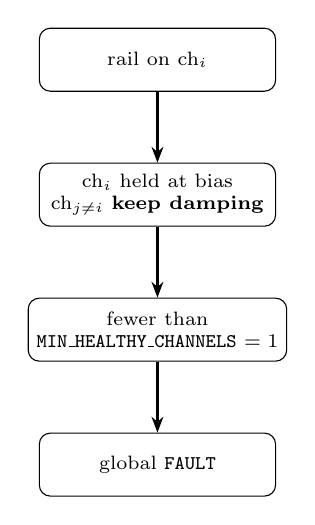
\begin{tikzpicture}[node distance=1.4cm]
        \node[blk, minimum width=3.0cm] (rail) {rail on ch$_i$};
        \node[blk, minimum width=3.0cm, below=0.9cm of rail] (dem)
          {ch$_i$ held at bias\\ch$_{j\neq i}$ \textbf{keep damping}};
        \node[blk, minimum width=3.0cm, below=0.9cm of dem] (q)
          {fewer than\\\texttt{MIN\_HEALTHY\_CHANNELS} $= 1$};
        \node[blk, minimum width=3.0cm, below=0.9cm of q] (f) {global \texttt{FAULT}};
        \draw[flow] (rail) -- (dem);
        \draw[flow] (dem) -- (q);
        \draw[flow] (q) -- (f);
      \end{tikzpicture}
    \end{column}
    \begin{column}{0.54\textwidth}
      \footnotesize
      \textbf{The problem.} \texttt{alpha} freezes all four channels on any one rail. One
      OSEM losing its flag stops \emph{all} damping, at the moment of
      largest excursion, which is what made the flag leave range.

      \vspace{2mm}
      \textbf{A quorum of one is not a guess}: the \texttt{zero} campaign measured one
      OSEM/coil pair damping the whole rigid body.

      \vspace{2mm}
      {\scriptsize\setlength{\tabcolsep}{4pt}
      \begin{tabular}{@{}ll>{\raggedright\arraybackslash}p{0.46\linewidth}@{}}
        \toprule
        condition & \texttt{alpha} & why \\
        \midrule
        rail & \textbf{demote} & local \emph{sensing} failure: that measurement
          is garbage \\
        runaway & global & not localisable: four loops, one body \\
        saturation & global & measurement fine, only the output clipped \\
        \bottomrule
      \end{tabular}}

      \vspace{2mm}
      Saturation is deliberately \emph{not} demoted: a saturated channel is
      still pushing the right way at full authority.
      \textbf{First fired on hardware under the eight-channel step}: ch2 railed, 3 of 4 kept
      damping, re-armed 2\,s later.
    \end{column}
  \end{columns}
\end{frame}
\note{alpha, the second file of that name, is alpha plus exactly one behavioural
change, so a bench comparison isolates it. It gives identical damping numbers to
alpha, because in a quiet lab nothing ever demotes. The whole change is dormant
until something goes wrong.

The problem: alpha freezes all four channels on any one rail. The stated reason was
that all four OSEMs sit on one rigid body so one blind sensor makes the optic's
position untrustworthy globally. True for reconstructing the optic's state, but
no version does that. They are four independent SISO loops. So all damping
stopped at the moment of largest excursion, which is exactly what made the flag
leave range in the first place.

The table is the design. A rail is a local sensing failure, so demote that
channel. A runaway is not localisable, so it stays global. Saturation stays
global deliberately: a saturated channel is still pushing the right way at full
authority, so parking it would remove damping at peak amplitude, the same mistake
this version exists to fix. It would also limit-cycle, since a channel demoted
for saturation immediately stops saturating.

Re-arming has three careful details. The filters are not reset, because
re-seeding a one-pole injects a step and the two-second hold is five time
constants of the highpass. The baseline is carried forward rather than
re-measured, because re-measuring would measure the event. And the gain ramps
back from zero.

It took until 2026-08-06 for this path to run on hardware for the first time.}

% ================================================================ 26
\begin{frame}{\texttt{beta}: stop re-measuring during the event}
  \begin{columns}[T]
    \begin{column}{0.48\textwidth}
      \centering
      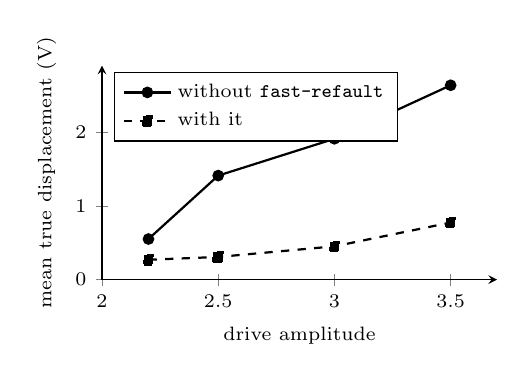
\begin{tikzpicture}
        \begin{axis}[width=6.6cm, height=4.3cm,
                     xlabel={drive amplitude}, ylabel={mean true displacement (V)},
                     xmin=2.0, xmax=3.7, ymin=0, ymax=2.9,
                     axis lines=left, legend pos=north west,
                     legend cell align=left, mark size=1.7pt]
          \addplot[thick, mark=*] coordinates
            {(2.2,0.550) (2.5,1.409) (3.0,1.908) (3.5,2.633)};
          \addlegendentry{without \texttt{fast-refault}}
          \addplot[thick, dashed, mark=square*] coordinates
            {(2.2,0.269) (2.5,0.307) (3.0,0.451) (3.5,0.773)};
          \addlegendentry{with it}
        \end{axis}
      \end{tikzpicture}\\
      {\scriptsize Simulator \emph{ground truth} over 300\,s, not the
      controller's own estimate.}
    \end{column}
    \begin{column}{0.5\textwidth}
      \footnotesize
      \textbf{The problem.} Every build before this one answers \emph{every} fault the same way: wait
      for all-clear, then recalibrate. That is \texttt{CALIBRATION\_S} of open
      loop at zero gain. Correct for a transient, wrong for a disturbance that
      has not gone away: the optic rings straight back up to the amplitude that
      faulted it.

      \vspace{2mm}
      \centering
      {\scriptsize
      \begin{tabular}{@{}lccc@{}}
        \toprule
        200\,s @ drive 2.5 & \% DAMPING & faults & locks \\
        \midrule
        earliest builds & 0.6\% & 1 & never \\
        with the 3 defect fixes & 4.1\% & 7 & never \\
        \textbf{with \texttt{fast-refault}} & \textbf{87.5\%} & \textbf{1} & \textbf{10.2\,s} \\
        \bottomrule
      \end{tabular}}

      \vspace{2mm}
      \raggedright
      \textbf{The fix is four lines.} If the previous engagement lasted under
      \texttt{FAST\_REFAULT\_S} $= 15$\,s, the cause is still present, so
      re-engage on the baseline already in hand. Bounded by
      \texttt{MAX\_BASELINE\_REUSE} $= 4$.

      \vspace{1mm}
      Found by stressing the simulator across clipping regimes, not by
      reading the code.
    \end{column}
  \end{columns}
\end{frame}
\note{Every version up to alpha answers every fault identically: wait for all-clear,
then recalibrate. Twenty seconds of open loop at zero gain. Exactly right for a
transient, exactly wrong for a disturbance that is still present, because during
those twenty seconds the optic rings back up to the amplitude that faulted it and
faults again on contact. The result is a supervisor-level feedback loop that
spends its life measuring instead of damping.

Over two hundred seconds of sustained clipping, alpha and alpha spend four percent of
samples damping across seven faults and never lock. With fast-refault that becomes 87.5 percent and
locks in ten seconds.

The plot is the optic itself, simulator ground truth rather than the controller's
own estimate, and the gap widens with drive amplitude.

The fix is four lines, bounded at four reuses so a stale baseline cannot persist.
And note how it was found: by stressing the rebuilt simulator across clipping
regimes, not by reading the code.

What it does not fix: at the highest drive, with 56 percent of samples clipping,
it still exhausts its reuses. That regime is a sensor problem, not a control
problem.}

% ================================================================ 28
\begin{frame}{Defect 4: a near-zero baseline makes noise look like a runaway}
  \begin{columns}[T]
    \begin{column}{0.50\textwidth}
      \footnotesize
      \rawdata\ Calibrated baselines at the eight-OSEM step, on the bench:

      \vspace{1mm}
      \centering
      {\scriptsize\setlength{\tabcolsep}{3pt}
      \begin{tabular}{@{}lccccc@{}}
        \toprule
        & a0 & a4 & a5 & a6 & a7 \\
        \midrule
        baseline (V) & 0.3109 & \textbf{0.0014} & 0.0801 & \textbf{0.0050} &
          \textbf{0.0020} \\
        $1.8\times$ & 0.560 & \textbf{0.0025} & 0.144 & \textbf{0.0090} &
          \textbf{0.0036} \\
        \bottomrule
      \end{tabular}}

      \vspace{2mm}
      \raggedright
      a4's own bandpassed output never left $\pm 0.01$\,V. Against a trip line
      of \textbf{0.0025\,V} that is \textbf{4$\times$ over}.

      \vspace{1mm}
      Measured peak ratios: a4 \textbf{3.98}, a6 \textbf{4.79}, a7
      \textbf{11.31}. All on a signal too small to see.
    \end{column}
    \begin{column}{0.47\textwidth}
      \footnotesize
      \goeswrong\ Two properties combine.

      \vspace{1mm}
      \begin{enumerate}\setlength{\itemsep}{1pt}
        \item An OSEM with no in-band signal \textbf{does not rail}. It sits
              mid-scale with a flat bandpassed output, so \texttt{auto-disable}
              never fires.
        \item Runaway is a \textbf{global} fault, because it is not localisable.
      \end{enumerate}

      \vspace{1mm}
      So a channel measuring its own noise takes the entire rig down:
      \alert{\textbf{ten whole-rig faults in 145\,s, nine of them naming a4, a6
      or a7.}}

      \vspace{2mm}
      \thefix\ \texttt{baseline-floor}, now in \texttt{delta}. At the end of every calibration,
      demote any channel whose baseline is under \textbf{10\% of the median}
      across enabled channels.

      \vspace{1mm}
      2026-08-06: a4/a6/a7 demoted at $t = 20.001$\,s, then \textbf{40\,s of
      unbroken \texttt{DAMPING} and zero faults} on the same eight OSEMs.
    \end{column}
  \end{columns}
\end{frame}
\note{The fourth defect, and the arithmetic on the left is the whole thing.

Every test downstream of calibration is a ratio against the baseline. a4
calibrated a floor of 1.4 millivolts against channel zero's 311. The runaway trip
line is 1.8 times that, which is 2.5 millivolts. a4's bandpassed output never
left plus or minus ten millivolts, which is four times over the line. The
measured peak ratios were 3.98 on a4, 4.79 on a6 and 11.31 on a7, all on a signal
far too small to see.

Two properties combine to make that fatal. An OSEM carrying no in-band signal
does not rail: it sits mid-scale with a flat bandpassed output, which an RMS
interlock reads as perfect stability, so auto-disable never fires. And runaway is
a global fault, because with four loops on one body "amplitude is growing under
feedback" does not say which loop is feeding it. So a channel measuring nothing
but its own noise takes the entire rig down. Ten whole-rig faults in a hundred
and forty-five seconds, nine of them naming a4, a6 or a7.

The fix is baseline-floor, and the number
that moved is the last line: the same eight OSEMs went from ten faults in 145
seconds to forty seconds of unbroken damping with zero faults.}

% ================================================================ 29
\begin{frame}{\texttt{sysid}: measuring which coil moves what}
  \begin{columns}[T]
    \begin{column}{0.46\textwidth}
      \centering
      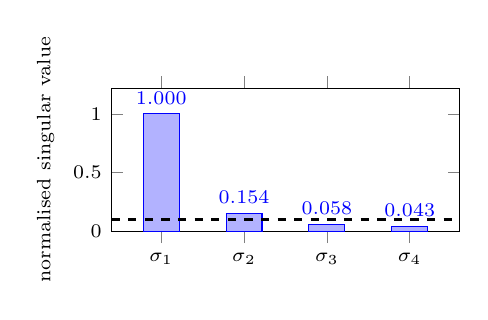
\begin{tikzpicture}
        \begin{axis}[width=6.0cm, height=3.4cm, ybar, bar width=13pt,
                     xtick={1,2,3,4},
                     xticklabels={$\sigma_1$,$\sigma_2$,$\sigma_3$,$\sigma_4$},
                     xmin=0.4, xmax=4.6, ymin=0, ymax=1.22,
                     ylabel={normalised singular value},
                     nodes near coords={\pgfmathprintnumber[fixed,zerofill,precision=3]{\pgfplotspointmeta}},
                     every node near coord/.append style={font=\scriptsize}]
          \addplot coordinates {(1,1.000) (2,0.154) (3,0.058) (4,0.043)};
          \draw[dashed, thick] (axis cs:0.4,0.10) -- (axis cs:4.6,0.10);
        \end{axis}
      \end{tikzpicture}\\
      {\scriptsize Dashed: the 10\% retention line.
       \textbf{Directions above it: 2}}
    \end{column}
    \begin{column}{0.5\textwidth}
      \footnotesize
      \texttt{KIND = "sysid"}. \textbf{Not a controller}: it damps nothing and
      closes no loop.

      \vspace{1.5mm}
      \textbf{Stepped sine, one coil at a time.} Drive one coil at a single
      frequency and measure only the response \emph{at that same frequency},
      which rejects everything else. While coil $j$ drives, no other coil is, so
      there is nothing to disentangle and \textbf{both the size and the timing of
      the response fall straight out}.

      \vspace{1.5mm}
      Only \textbf{4 of 12} frequencies were usable: ch2 railed in
      \textbf{17 of 48} steps, and two survivors are ambient-dominated.

      \vspace{1.5mm}
      \textbf{\texttt{sysid}.1 (multisine) failed outright}: ch2 railed in \textbf{all 4}
      passes, and pass 1 ran at \textbf{14.8\,Hz} effective against
      $\sim$252\,Hz, giving a spurious $\sim$\textbf{4700\,V/V} against
      $\sim$70.

      \vspace{1.5mm}
      \textbf{One cause for both:} open loop, nothing damping, ch2 clips.
      \textbf{And the rank check is superseded}: the ringdown finds
      \textbf{three} modes, and the full refit puts the allocator at
      $3 \times 4$, cond \textbf{1.41}.
    \end{column}
  \end{columns}
\end{frame}
\note{sysid is not a controller. It declares KIND equals sysid, exposes no
Controller class, damps nothing, and both the harness and the bench runner refuse
to simulate it.

What it does is drive one coil at a time with a sine and record what all the
OSEMs do, recovering the actuation matrix by lock-in detection. Why stepped sine
rather than something cleverer: while coil j is driving, no other coil is. There
is nothing to disentangle, no matrix to invert, and both quadratures come out of
the lock-in together, so magnitude and phase are measured rather than inferred.

It passed its own rank check: two directions above ten percent.

But be honest about the caveat. Only four of twelve frequencies were usable,
because channel two railed in seventeen of forty-eight steps, and two of those
four are ambient-dominated rather than drive-dominated. It is a valid measurement
on a quarter of the sweep.

The multisine variant failed outright. Both failures share one cause: open loop,
nothing damping, so the optic rings up and channel two clips. Closed-loop dither
is the way past it, and it is still on the open list.}

% ================================================================ 30
\begin{frame}{The DC actuation matrix, and the conclusion it will not support}
  \begin{columns}[T]
    \begin{column}{0.55\textwidth}
      \centering
      {\scriptsize\setlength{\tabcolsep}{3pt}
      \begin{tabular}{@{}lrrrr|rrrr@{}}
        \toprule
        & \multicolumn{4}{c|}{coils 0--3} & \multicolumn{4}{c}{coils 4--7} \\
        \midrule
        a0 & $-105$ & $-107$ & $-48$ & $+19$ & $-29$ & $-21$ & $-28$ & $-26$ \\
        a1 & $-49$ & $-68$ & $-33$ & $+18$ & $+5$ & $+7$ & $+4$ & $+8$ \\
        a2 & $+35$ & $+66$ & $+213$ & $-141$ & $-25$ & $-22$ & $-13$ & $-26$ \\
        a3 & $+36$ & $+14$ & $+58$ & $-51$ & $-1$ & $-2$ & $+2$ & $-1$ \\
        \midrule
        a4 & $+0$ & $+2$ & $+2$ & $+1$ & $+8$ & $+8$ & $+2$ & $+1$ \\
        a5 & $+4$ & $+0$ & $+0$ & $-6$ & $-0$ & $-7$ & $-1$ & $+8$ \\
        a6 & $+1$ & $+4$ & $+2$ & $+3$ & $+3$ & $+3$ & $+4$ & $+6$ \\
        a7 & $-0$ & $+3$ & $+1$ & $+0$ & $+1$ & $-1$ & $+6$ & $+7$ \\
        \bottomrule
      \end{tabular}}\\
      {\scriptsize $d(\text{counts}_i)/d(\text{bias}_j)$, one coil stepped at a
      time, bench 2026-08-04.}
    \end{column}
    \begin{column}{0.43\textwidth}
      \centering
      {\footnotesize \textbf{Block means of $|$response$|$}}\\[1mm]
      {\footnotesize
      \begin{tabular}{@{}lcc@{}}
        \toprule
        & coils 0--3 & coils 4--7 \\
        \midrule
        sensors 0--3 & \textbf{66} & \textbf{14} \\
        sensors 4--7 & 2 & \textbf{4} \\
        \bottomrule
      \end{tabular}}

      \vspace{2mm}
      \scriptsize
      \raggedright
      \textbf{Coils 4--7 work}: they move a0--a3 by $\sim$25\,counts/V.
      \textbf{Sensors a4--a7 respond to nothing}, $\leq 8$\,counts/V.

      \vspace{1.5mm}
      We read that as ``a4--a7 are not wired''. It was wrong. A DC slope
      against a fixed threshold cannot separate \emph{no sensor} from \emph{a
      working sensor with small gain}. \textbf{Wrong statistic, not wrong data.}

      \vspace{1.5mm}
      Their own diagonals are $+8 / +4 / +7$ against a block mean of
      \textbf{4}. Those signs are coin flips, and \textbf{a wrong sign pumps},
      so the 500000-baud step and \texttt{delta} ship a4/a6/a7 at \textbf{zero gain}.

      \vspace{1.5mm}
      a3: the common-mode sweep read $+43$\,counts/V, coil3 $\to$ a3 alone
      $-51$. \textbf{Common-mode slopes are not per-coil slopes.}
    \end{column}
  \end{columns}
\end{frame}
\note{Step each coil's bias one at a time and record how every sensor's resting
count moves. That gives an eight-by-eight DC actuation matrix in counts per volt.

Read the two-by-two block summary. Within the wired block the mean response
magnitude is 66 counts per volt. Coils four to seven onto the wired sensors is
14, so those coils demonstrably work. But nothing moves sensors a4 to a7 by more
than eight counts per volt.

We concluded that the four extra OSEMs were not connected, and wrote that into
the repository. It was wrong. The shape of the mistake is the part to keep: a DC
slope compared against a fixed threshold cannot tell a sensor that is absent from
a sensor that is present with a small gain. Nothing here is bad data. Every number
in this table is real.

There is a second thing this table cannot support. Read the diagonal of the
lower-right block: plus eight, plus four, plus seven, in a block whose mean
absolute response is four. Those diagonals are at or barely above the noise of
the block they sit in, and a sign read off a number like that is a coin flip
dressed as a measurement. A wrong-signed channel pumps, so the 500000-baud step and delta enable all
three as sensors at exactly zero gain.

One trap worth calling out, because it nearly cost a sign error. A common-mode
sweep, moving all four coils together, read plus 43 counts per volt for sensor
a3. Coil three onto a3 alone is minus 51. Opposite sign.}

% ================================================================ 31
\begin{frame}{All eight \emph{are} wired: in-band against out-of-band}
  \begin{columns}[T]
    \begin{column}{0.48\textwidth}
      \centering
      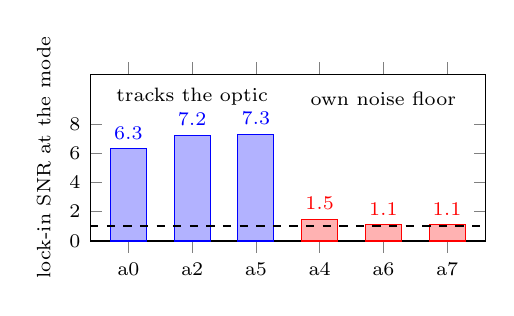
\begin{tikzpicture}
        \begin{axis}[width=6.6cm, height=3.7cm, ybar, bar width=13pt,
                     xtick={1,2,3,4,5,6},
                     xticklabels={a0,a2,a5,a4,a6,a7},
                     xmin=0.4, xmax=6.6, ymin=0, ymax=11.4,
                     ytick={0,2,4,6,8},
                     ylabel={lock-in SNR at the mode},
                     nodes near coords={\pgfmathprintnumber[fixed,zerofill,precision=1]{\pgfplotspointmeta}},
                     every node near coord/.append style={font=\scriptsize},
                     every axis plot post/.append style={bar shift=0pt}]
          \addplot coordinates {(1,6.3) (2,7.2) (3,7.3)};
          \addplot coordinates {(4,1.5) (5,1.1) (6,1.1)};
          \draw[dashed, thick] (axis cs:0.4,1.0) -- (axis cs:6.6,1.0);
          \node[font=\scriptsize, anchor=south] at (axis cs:2,8.6)
            {tracks the optic};
          \node[font=\scriptsize, anchor=south] at (axis cs:5,8.6)
            {own noise floor};
        \end{axis}
      \end{tikzpicture}\\
      {\scriptsize Lock-in on the two long 8-channel logs (118\,s, 148\,s) at
       the mode frequencies. Dashed: SNR $= 1$.}
    \end{column}
    \begin{column}{0.50\textwidth}
      \footnotesize\raggedright
      \textbf{All eight OSEMs are electrically connected}, confirmed on a
      scope. The split is \emph{in band} against \emph{out of band}:

      \vspace{1.5mm}
      {\scriptsize\setlength{\tabcolsep}{4pt}
      \begin{tabular}{@{}l r>{\raggedright\arraybackslash}p{0.42\linewidth}@{}}
        \toprule
        & \multicolumn{2}{@{}l}{power in 0.4--3\,Hz} \\
        \midrule
        a0--a3 & 77--99\% & the three modes \\
        a5 & 22--71\% & in band here, not in the residue fit \\
        a4, a6, a7 & 0.1--9\% & a narrow \textbf{6.19\,Hz} line
          (12.4\,Hz harmonic on a7) \\
        \bottomrule
      \end{tabular}}

      \vspace{1.5mm}
      \textbf{Not an Arduino or sampling problem.} a3 is read
      \emph{immediately before} a4 and carries a large 1.64\,Hz signal, yet
      $r(\mathrm{a4},\mathrm{a3}) = -0.029 / +0.004$. a5, read straight
      \emph{after} a4, is clean.

      \vspace{1.5mm}
      \alert{\textbf{The cause of the low gain is NOT established.}} ``Flags
      outside the linear region'' is \textbf{unsupported}: a4 rests at
      \textbf{567.5} counts against mid-scale \textbf{511.5} with a
      \textbf{30-count swing}, nowhere near an end.
    \end{column}
  \end{columns}
\end{frame}
\note{The correction, and it matters because two earlier claims in this
repository were wrong.

First: all eight OSEMs are electrically connected. Confirmed on an oscilloscope.
The claim that a4 to a7 were not wired was simply wrong.

The split is in-band against out-of-band, and the table has it. What the table
does not say is that a4, a6 and a7 carry real signal, raw standard deviations of
13 to 105 counts, and do move on a hard kick, seen on a scope. They are not dead.

Second correction, and this one is a retraction: we do not know why. The story was that their flags sit outside
the linear partial-shadow region. The resting counts do not support it. a4 sits
at 567.5 counts against a mid-scale of 511.5, with a thirty-count swing. That is
inside its range, not pinned at an end. a7 is at 734.7 and a6 at 860.6, higher
but still off the rail. So: the low in-band gain is measured, the cause is open,
and the honest thing is to say so.

Head off the obvious question about the Arduino. a3 is read immediately before a4
and carries a large clean signal, the strongest possible source for multiplexer
leakage, and the correlation between a4 and a3 is minus 0.029 and plus 0.004 on
the two runs. Nothing leaks. And a5, read straight after a4, is clean.

a5 is marked contested and gets its own slide, because two measurements
disagree about it and the newer one wins.

The methodological point: the original call rested on a DC-response threshold and
a raw time-domain correlation. Both are blind to a small coherent signal. The
spectral test found the answer immediately on exactly the same data. Wrong
statistic, not wrong data.}

% ================================================================ 34
\begin{frame}{Defect 5: the runaway breaker was asking the wrong question}
  \centering
  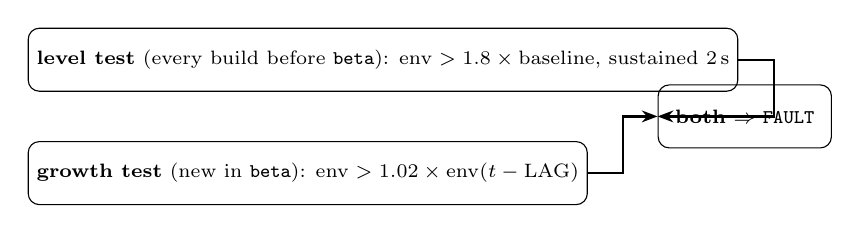
\begin{tikzpicture}[font=\scriptsize]
    \node[blk, minimum width=6.8cm, anchor=west] (lev) at (0,0.72)
      {\textbf{level test} (every build before \texttt{beta}):
       $\mathrm{env} > 1.8 \times \mathrm{baseline}$, sustained 2\,s};
    \node[blk, minimum width=6.8cm, anchor=west] (grow) at (0,-0.72)
      {\textbf{growth test} (new in \texttt{beta}):
       $\mathrm{env} > 1.02 \times \mathrm{env}(t - \mathrm{LAG})$};
    \node[blk, minimum width=2.2cm, anchor=west] (and) at (8.0,0)
      {\textbf{both} $\Rightarrow$ \texttt{FAULT}};
    \draw[flow] (lev.east) -- ++(0.45,0) |- (and.west);
    \draw[flow] (grow.east) -- ++(0.45,0) |- (and.west);
  \end{tikzpicture}

  \vspace{4mm}
  \begin{columns}[T]
    \begin{column}{0.47\textwidth}
      \footnotesize
      A \textbf{runaway} is the loop pumping energy \emph{in}: the envelope
      \textbf{grows}.

      \vspace{1mm}
      A \textbf{ringdown} is a large but \textbf{falling} envelope: the loop
      \emph{succeeding}.

      \vspace{2mm}
      A level test cannot tell them apart. After a kick it trips on a
      timer, every \texttt{RUNAWAY\_SUSTAIN\_S}, all the way down the ringdown.
    \end{column}
    \begin{column}{0.49\textwidth}
      \footnotesize
      \textbf{This defect was in every version back to \texttt{zero}.} The build just before \texttt{beta} merely re-engaged
      fast enough to hit it repeatedly, which is how it was found.

      \vspace{2mm}
      \texttt{RUNAWAY\_GROWTH\_FRAC = 1.02} gives 2\% of headroom so envelope
      noise alone cannot read as growth.

      \vspace{2mm}
      \texttt{RUNAWAY\_TREND\_LAG\_S = 2.0} was chosen before the mode
      frequencies were known. That turns out to be the next defect, and it took
      three more versions to find.
    \end{column}
  \end{columns}
\end{frame}
\note{The best single result in the project, and it needs three slides.

The runaway breaker, from the zero build right up to beta, was a level test: is the envelope above
1.8 times baseline, sustained two seconds. That sounds reasonable and it is
wrong, for a reason obvious once stated.

A runaway means the loop is pumping energy in, which means the envelope is
growing. A large but decaying envelope means the loop is succeeding. A level test
cannot distinguish those. So after a kick, while the optic is ringing down under
perfectly good control, the breaker trips on a timer and keeps tripping, every
two seconds, all the way down, until the amplitude happens to fall under the line
by luck.

beta keeps the level test and adds a growth test: the envelope must also exceed
where it was one lag ago, by two percent. Both conditions, both sustained.

The thing to appreciate: this defect was present in every version back to the zero build. It
took until the build just before beta to find, and only because that build re-engaged fast enough after a fault
to make the pattern visible.

Note the last box, because it is a trap being set. The lag was picked at two
seconds before anybody had measured the mode frequencies. That is the next defect
and it took three more versions.}

% ================================================================ 35
\begin{frame}{The defect on the bench: the envelope \emph{falling} through every fault}
  \centering
  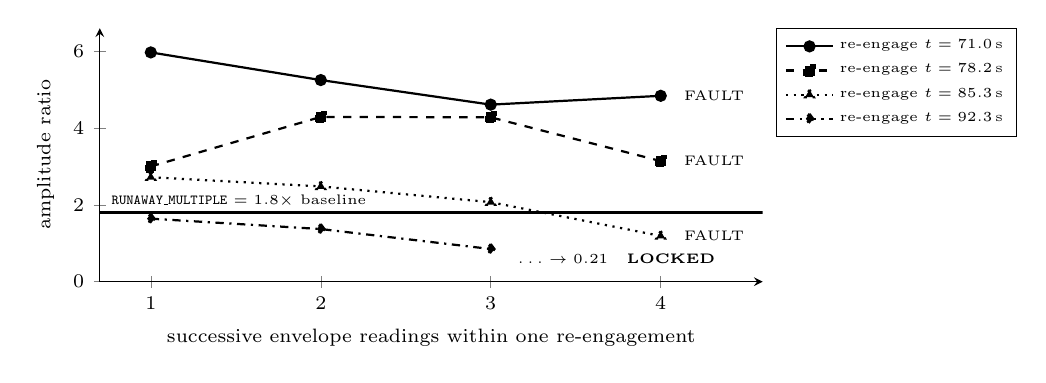
\begin{tikzpicture}
    \begin{axis}[width=10.0cm, height=4.8cm,
                 xlabel={successive envelope readings within one re-engagement},
                 ylabel={amplitude ratio},
                 xmin=0.7, xmax=4.6, ymin=0, ymax=6.6,
                 xtick={1,2,3,4}, axis lines=left,
                 legend style={at={(1.02,1.0)}, anchor=north west, font=\tiny},
                 legend cell align=left, mark size=1.8pt]
      \addplot[thick, mark=*] coordinates {(1,5.97) (2,5.25) (3,4.61) (4,4.84)};
      \addlegendentry{re-engage $t=71.0$\,s}
      \addplot[thick, mark=square*, dashed] coordinates {(1,3.00) (2,4.29) (3,4.28) (4,3.14)};
      \addlegendentry{re-engage $t=78.2$\,s}
      \addplot[thick, mark=triangle*, dotted] coordinates {(1,2.72) (2,2.48) (3,2.07) (4,1.19)};
      \addlegendentry{re-engage $t=85.3$\,s}
      \addplot[thick, mark=diamond*, dashdotted] coordinates {(1,1.64) (2,1.37) (3,0.85)};
      \addlegendentry{re-engage $t=92.3$\,s}
      \draw[thick] (axis cs:0.7,1.8) -- (axis cs:4.6,1.8);
      \node[font=\tiny, anchor=south west, fill=white, inner sep=1pt]
        at (axis cs:0.75,1.85)
        {\texttt{RUNAWAY\_MULTIPLE} $= 1.8 \times$ baseline};
      \node[font=\tiny, anchor=west] at (axis cs:4.08,4.84) {FAULT};
      \node[font=\tiny, anchor=west] at (axis cs:4.08,3.14) {FAULT};
      \node[font=\tiny, anchor=west] at (axis cs:4.08,1.19) {FAULT};
      \node[font=\tiny, anchor=west] at (axis cs:3.10,0.60)
        {$\ldots \to 0.21$\quad \textbf{LOCKED}};
    \end{axis}
  \end{tikzpicture}

  \vspace{-1mm}
  {\footnotesize Measured on \textbf{the build just before \texttt{beta}: hardware, 240\,s, three kicks}:
  \textbf{ten faults}, and the envelope was \emph{falling} through them.
  Only the re-engagement that happened to start at 1.64, just under the
  line, survived.}
\end{frame}
\note{Here is the defect caught in the act, on hardware. The build just before beta, two hundred and
forty seconds, three kicks, ten faults. Each line is one re-engagement after a
fault, and the y-axis is the amplitude ratio the breaker is watching.

Look at the first line. The loop re-engages at 5.97 times baseline, brings it to
5.25, then 4.61. It is working. Then the breaker faults it anyway, because the
level was above 1.8 the whole time. Same on the second and third. The optic is
being damped and the supervisor keeps taking the controller away from it.

The fourth line is the giveaway. It re-engaged at 1.64, just under the line, so
the breaker never armed, and that engagement ran all the way down to 0.21 and
locked. The only thing separating the successful engagement from the three
failures is where it happened to start relative to an arbitrary threshold.}

% ================================================================ 36
\begin{frame}{\texttt{beta}: what the growth test bought}
  \begin{columns}[T]
    \begin{column}{0.54\textwidth}
      \centering
      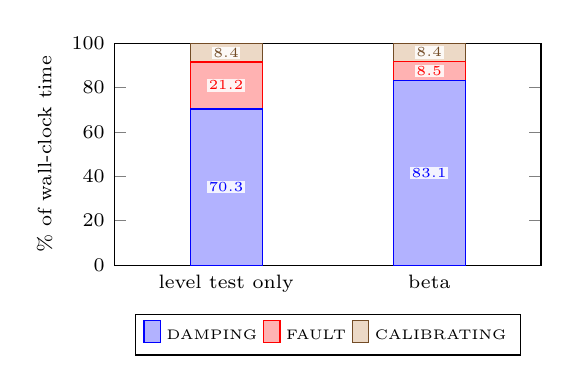
\begin{tikzpicture}
        \begin{axis}[width=7.0cm, height=4.4cm, ybar stacked, bar width=26pt,
                     symbolic x coords={level test only, beta},
                     xtick=data, ymin=0, ymax=100,
                     ylabel={\% of wall-clock time},
                     x tick label style={font=\scriptsize},
                     legend style={at={(0.5,-0.22)}, anchor=north, legend columns=3,
                                   font=\tiny},
                     nodes near coords={\pgfmathprintnumber[fixed,zerofill,precision=1]{\pgfplotspointmeta}},
                     every node near coord/.append style={font=\tiny,
                       fill=white, fill opacity=0.85, text opacity=1,
                       inner sep=0.6pt},
                     enlarge x limits=0.55]
          \addplot coordinates {(level test only,70.3) (beta,83.1)};
          \addlegendentry{DAMPING}
          \addplot coordinates {(level test only,21.2) (beta,8.5)};
          \addlegendentry{FAULT}
          \addplot coordinates {(level test only,8.4) (beta,8.4)};
          \addlegendentry{CALIBRATING}
        \end{axis}
      \end{tikzpicture}\\
      {\scriptsize The same build with and without the growth test, on the same
      240\,s three-kick schedule.}
    \end{column}
    \begin{column}{0.44\textwidth}
      \footnotesize
      \centering
      {\footnotesize
      \begin{tabular}{@{}lcc@{}}
        \toprule
        same 3-kick schedule & faults & locks \\
        \midrule
        level test only & \textbf{10} & 4 \\
        \textbf{\texttt{beta}} & \textbf{4} & \textbf{4} \\
        \bottomrule
      \end{tabular}}

      \vspace{2mm}
      \raggedright
      \textbf{\texttt{beta} re-locked after \emph{every} kick}, at
      $t = 31.3 / 83.8 / 151.3 / 205.3$\,s.

      \vspace{2mm}
      \texttt{beta}'s \texttt{FAULT} time is \textbf{20.2\,s} $=$ the mandatory
      5\,s all-clear $\times$ 4 recoveries. \textbf{Cost, not thrash.}

      \vspace{2mm}
      \textbf{83.1\% is still the best \texttt{DAMPING} fraction on record.}
      Every later comparison has to say what kick schedule it ran.
    \end{column}
  \end{columns}
\end{frame}
\note{The same build with and without the growth test, on the same three-kick
schedule, so this is a controlled comparison rather than two different programs.

Without it: 21 percent of the run in FAULT across ten faults. With it: 8.5
percent across four, and damping time up to 83.1 percent, while re-locking after
every single kick.

What is left is understood rather than mysterious. 8.5 percent of 238 seconds is
20.2 seconds, which is exactly five seconds of mandatory all-clear times four
recoveries. Cost, not thrash.

And the caution I want standing for the rest of the deck: 83.1 percent is still
the best damping fraction anyone has measured here, on this schedule. Later runs
used different kick schedules, so any comparison against it has to say which.}

% ================================================================ 37
\begin{frame}{Defect 6: two estimators, one inverted conclusion}
  \begin{columns}[T]
    \begin{column}{0.52\textwidth}
      \centering
      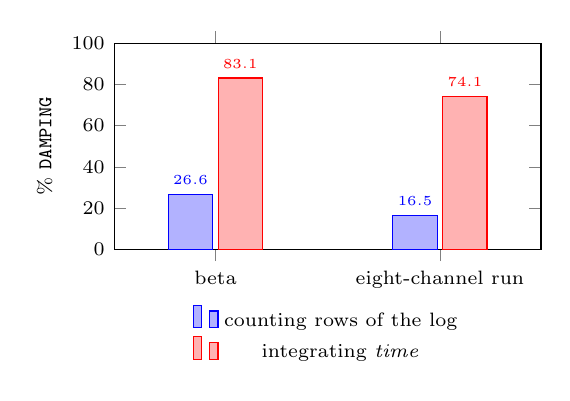
\begin{tikzpicture}
        \begin{axis}[width=7.0cm, height=4.2cm, ybar, bar width=16pt,
                     symbolic x coords={beta, eight-channel run},
                     xtick=data, ymin=0, ymax=100,
                     ylabel={\% \texttt{DAMPING}},
                     x tick label style={font=\scriptsize},
                     legend style={at={(0.5,-0.24)}, anchor=north,
                                   legend columns=1, draw=none, fill=none},
                     nodes near coords={\pgfmathprintnumber[fixed,zerofill,precision=1]{\pgfplotspointmeta}},
                     every node near coord/.append style={font=\tiny},
                     enlarge x limits=0.45]
          \addplot coordinates {(beta,26.6) (eight-channel run,16.5)};
          \addlegendentry{counting rows of the log}
          \addplot coordinates {(beta,83.1) (eight-channel run,74.1)};
          \addlegendentry{integrating \emph{time}}
        \end{axis}
      \end{tikzpicture}\\
      {\scriptsize Identical logs and state column. Only the weighting differs.}
    \end{column}
    \begin{column}{0.46\textwidth}
      \footnotesize\raggedright
      \rawdata\ The eight-channel run's \textbf{74.1\%} (time) against
      \texttt{beta}'s \textbf{26.6\%} (rows) $= 2.8\times$.

      \vspace{1.5mm}
      \goeswrong\ That reads as ``the newer build nearly tripled the damping
      duty''. The two halves came from different estimators. \textbf{Like for
      like, either way, \texttt{beta} wins}: time \textbf{83.1} vs 74.1; rows
      \textbf{26.6} vs 16.5.

      \vspace{1.5mm}
      \textbf{Why rows lie.} The loop samples at \textbf{24--26\,Hz} while
      actuating and \textbf{341--351\,Hz} otherwise, because only actuating pays
      the serial round trip. A row count weights each state by how \emph{fast}
      it samples.

      \vspace{1.5mm}
      The distortion is not constant: rows understate \texttt{DAMPING} by
      $3.1\times$ on \texttt{beta} and $4.5\times$ on the other. Row-based
      figures are not comparable to \emph{each other} either.

      \vspace{1.5mm}
      \thefix\ Integrate timestamps.
    \end{column}
  \end{columns}
\end{frame}
\note{A slide about a mistake, because it is the most transferable thing in the
deck. This is a defect in the analysis rather than in the controller, and it
nearly shipped.

Both bar groups come from exactly the same logs and the same state column. The
only difference is the weighting: short bars count rows, tall bars integrate
timestamps.

The mistake was to divide one by the other, which makes the newer build look like
it nearly tripled the damping duty. Measured the same way, either way you like,
beta is ahead.

The mechanism is the loop-rate result from earlier. The controller only pays the
serial round trip while actuating, so it samples at 24 to 26 hertz while damping
and around 345 hertz otherwise. A row count therefore weights each state by how
fast it happens to sample, which is a measure of how little the controller was
doing.

And the distortion is not a constant you could correct for, so row-based duty
cycles are not comparable to each other either, before you even mix estimators.

How it was caught: not by a clever check, just by noticing that two numbers being
compared came from different places.}

% ================================================================ 38
\begin{frame}{\texttt{delta}: a clipped loop is weakened, not broken}
  \begin{columns}[T]
    \begin{column}{0.34\textwidth}
      \centering
      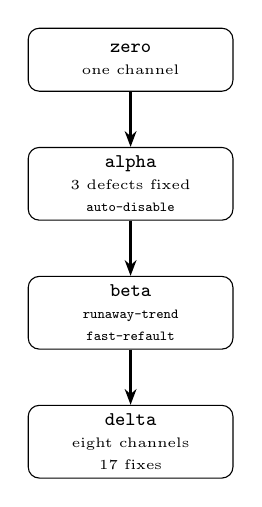
\begin{tikzpicture}[font=\scriptsize, node distance=7mm]
        \node[blk, minimum width=2.6cm] (z) {\texttt{zero}\\{\tiny one channel}};
        \node[blk, minimum width=2.6cm, below=of z] (al) {\texttt{alpha}\\{\tiny 3 defects fixed}\\{\tiny \texttt{auto-disable}}};
        \node[blk, minimum width=2.6cm, below=of al] (be) {\texttt{beta}\\{\tiny \texttt{runaway-trend}}\\{\tiny \texttt{fast-refault}}};
        \node[blk, minimum width=2.6cm, below=of be] (de) {\textbf{\texttt{delta}}\\{\tiny eight channels}\\{\tiny 17 fixes}};
        \draw[flow] (z) -- (al);
        \draw[flow] (al) -- (be);
        \draw[flow] (be) -- (de);
      \end{tikzpicture}\\[1mm]
      {\scriptsize Four kept rungs. Further builds ran between them and are in
      version control only.}
    \end{column}
    \begin{column}{0.64\textwidth}
      \footnotesize
      \textbf{The fix.} Earlier builds faulted the whole rig after 30
      consecutive samples with an output pinned at its limit. But
      \textbf{clipping removes push in one direction only}: an output stuck at
      the top of its range can still pull all the way down at full strength. A
      clipped loop is a \textbf{weakened} loop, not a broken one, and it is
      usually the thing bringing the mirror back.

      \vspace{2mm}
      \centering
      {\scriptsize $\texttt{sat\_trip} = (\text{streak} > 30)
         \ \wedge\ \neg(\text{amplitude falling})$}

      \vspace{2mm}
      \raggedright
      \textbf{The same level-against-trend correction the runaway breaker got,
      one interlock over.} Same history, same lag, so ``falling'' means one
      thing to both.

      \vspace{2mm}
      \textbf{And a coupling worth knowing.} Nudging a coil's resting current
      \emph{is} a force step: it rings the pendulum inside the band both trend
      tests read. So a nudge \textbf{invalidates} the history instead of
      suspending the interlocks, which would open a 16\,s hole every 15\,s.
    \end{column}
  \end{columns}
\end{frame}
\note{The named ladder on the left, because this is the point where it is worth
showing. Four kept rungs: zero, alpha, beta, delta. Other builds ran between
them and are in version control only; I am not going to pretend the project went
in four clean steps.

The fix itself generalises beta's insight to the neighbouring interlock. Earlier
builds faulted the whole rig after thirty consecutive samples with an output
pinned. But clipping removes push in one direction only: an output stuck at the
top of its range can still pull all the way down at full strength. So a clipped
loop is a weakened loop, not a broken one, and it is usually the thing bringing
the mirror back. Faulting replaces a half-strength actuator with a frozen one,
which is strictly worse.

So the trip now needs the streak and a non-falling amplitude, reusing the same
history and the same lag so that falling means exactly one thing across both
interlocks.

And one coupling worth knowing. Nudging a coil's resting current is a force step:
it rings the pendulum inside the band both trend tests read. Suspending the
interlocks for that would open a sixteen second hole every fifteen seconds. So
instead a nudge invalidates the history it would have corrupted.}

% ================================================================ 39
\begin{frame}{\texttt{bias-trim} inside a live loop}
  \begin{columns}[T]
    \begin{column}{0.49\textwidth}
      \centering
      {\scriptsize\setlength{\tabcolsep}{4pt}
      \begin{tabular}{@{}lll@{}}
        \toprule
        trim step & total offset & verdict \\
        \midrule
        ch3 $\to$ 0.50\,V & $576 \to 560$ & kept \\
        ch3 $\to$ 0.75\,V & $560 \to 532$ & kept \\
        ch3 $\to$ 1.00\,V & $532 \to 507$ & kept \\
        ch1 $\to$ 0.50\,V & $507 \to \mathbf{472}$ & kept \\
        ch3 $\to$ 1.25\,V & $472 \to 564$ & reverted \\
        ch1 $\to$ 0.75\,V & $489 \to 477$ & kept \\
        ch1 $\to$ 1.00\,V & $477 \to 481$ & reverted \\
        ch0 $\to$ 0.50\,V & $501 \to 522$ & reverted \\
        \bottomrule
      \end{tabular}}\\[1.5mm]
      {\scriptsize Total $|$offset from mid-scale$|$, four OSEMs, counts.}
    \end{column}
    \begin{column}{0.49\textwidth}
      \scriptsize\raggedright
      \textbf{Accept-or-revert earns its keep.} \textbf{3 of 8} steps made the
      \emph{rig} worse and were frozen. ch3 at 1.25\,V cost \textbf{92 counts}
      in one step: four coils, two DOF.

      \vspace{1.5mm}
      \textbf{More faults, no thrash.} 35.7\,s of \texttt{FAULT} over 7 trips is
      \textbf{5.1\,s each}, the mandatory \texttt{FAULT\_CLEAR\_SUSTAIN\_S}, as
      \texttt{beta}'s 5.05\,s.

      \vspace{1.5mm}
      \textbf{ch3 caused 7 of the 8 events} (ch1 and ch2 one each). It
      has the \textbf{weakest coil} at $-51$\,counts/V against ch0's $-105$ and
      ch2's $+213$, and it is the channel the trim stepped three times.
      \textbf{A bias step is a force step.} \emph{Trim the weakest coil last.}

      \vspace{1.5mm}
      \textbf{\texttt{soft-saturation} never fired}: every trip was the
      runaway breaker. But \texttt{auto-disable} did, for the first time on
      hardware: ch2 railed, \textbf{3 of 4} kept damping, re-armed 2\,s later.
    \end{column}
  \end{columns}
\end{frame}
\note{the eight-channel step ran on hardware on the same 240-second three-kick schedule as beta, and
it is the first time bias-trim ran inside a live damping loop.

Eight steps were attempted, five kept, three reverted and frozen. The reverts are
the point: each helped its own channel and made the total offset worse. ch3 at
1.25 volts cost 92 counts in a single step, and without accept-or-revert that
step would have stood. Best total offset reached was 472 counts from 576.

None of the extra faults is thrash. Thirty-five point seven seconds of FAULT over
seven global trips is 5.1 seconds each, exactly the mandatory all-clear hold. beta
was 5.05.

And we know why there were more. Channel three caused seven of the eight events.
It has the weakest coil in the whole DC actuation matrix, minus 51 counts per
volt against minus 105 on ch0 and plus 213 on ch2, so it has the least authority
to arrest a kick. It is also the channel the trim stepped three times, and a bias
step is a force step: the trim was perturbing the axis with the least margin.
That is actionable. Trim the weakest channel last, not first.

Finally, the caveat that matters most. soft-saturation, the fix the eight-channel step exists for,
never fired once. Every trip was the runaway breaker. What did get confirmed for
the first time is auto-disable, from alpha: channel two railed, the other three kept
damping, and it re-armed two seconds later.}

% ================================================================ 40
\begin{frame}{\texttt{baseline-floor}: the guard eight channels needed}
  \begin{columns}[T]
    \begin{column}{0.50\textwidth}
      \centering
      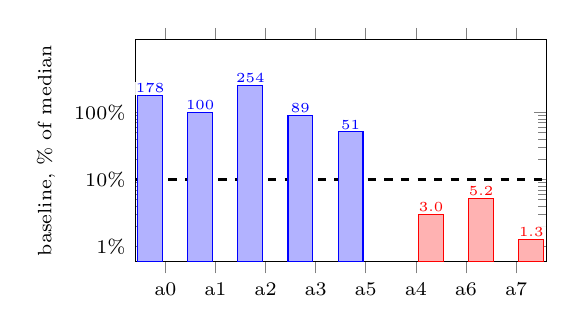
\begin{tikzpicture}
        \begin{axis}[width=6.8cm, height=4.4cm, ybar, bar width=9pt,
                     ymode=log, log origin=infty, ymin=0.6, ymax=1200,
                     xtick={1,2,3,4,5,6,7,8},
                     xticklabels={a0,a1,a2,a3,a5,a4,a6,a7},
                     xmin=0.4, xmax=8.6,
                     ytick={1,10,100},
                     yticklabels={1\%,10\%,100\%},
                     ylabel={baseline, \% of median},
                     nodes near coords, point meta=explicit symbolic,
                     every node near coord/.append style={font=\tiny,
                       fill=white, fill opacity=0.9, text opacity=1,
                       inner sep=0.8pt}]
          \draw[dashed, very thick] (axis cs:0.4,10) -- (axis cs:8.6,10);
          \addplot coordinates {(1,178) [178] (2,100) [100] (3,254) [254]
                                (4,89) [89] (5,51.3) [51]};
          \addplot coordinates {(6,3.0) [3.0] (7,5.2) [5.2] (8,1.3) [1.3]};
        \end{axis}
      \end{tikzpicture}\\
      {\scriptsize Dashed: \texttt{BASELINE\_FLOOR\_FRAC} $= 10\%$ of the median
       over \emph{enabled} channels, 2026-08-06. \textbf{It sits in an empty
       $10\times$ gap}: 5.2\% (worst dead) to 51.3\% (a5).}
    \end{column}
    \begin{column}{0.48\textwidth}
      \scriptsize\raggedright
      \textbf{The rule.} At the end of every calibration, a channel whose
      baseline is under 10\% of the \textbf{median} across enabled channels is
      demoted exactly as \texttt{auto-disable} demotes a railed one.

      \vspace{1.5mm}
      \textbf{Median, not mean, and that is the whole safety argument.} The
      largest baseline is always $\geq$ the median $>$ the threshold, so
      \textbf{at least one channel always survives}: no quorum arithmetic. And
      if \emph{most} of the rig is dead the median \emph{is} a dead channel, the
      threshold collapses, and the guard does nothing, rather than demoting six
      on the word of two.

      \vspace{1.5mm}
      \textbf{Relative, not absolute}, because an absolute floor in volts would
      depend on the seismic background and each OSEM's alignment. On a quieter
      night a real channel and a dead one fall together.

      \vspace{1.5mm}
      \textbf{And note what a config switch did \emph{not} do.} Those three were
      switched off in the configuration and still had to be demoted: the runaway
      breaker gates on \texttt{healthy}, not on \texttt{enabled}.
      Switching a channel off does not take it out of the interlocks.
    \end{column}
  \end{columns}
\end{frame}
\note{The eight-OSEM failure mode fixed, in a two-line rule.

Two design points behind it. Relative rather than a level in volts, because an
absolute floor would depend on the seismic background and each OSEM's alignment:
on a quieter night a real channel and a dead one fall together.

Median rather than mean, and that buys a safety property outright. The largest
enabled baseline is always at least the median, which is by definition above ten
percent of the median, so at least one channel always survives. No quorum
arithmetic needed. The dual case is just as deliberate: if most of the rig is
signal-less, the median is itself a dead channel, the threshold collapses toward
zero, and the guard does nothing. That is the right failure, because a reference
that has been captured cannot tell you which half is broken.

The threshold is not fine-tuned. The worst dead channel sits at 5.2 percent of
the median and a5, the weakest real one, at 51.3. Ten percent sits in an empty
ten-fold gap. And it is biased toward keeping: demoting a good sensor costs one
loop, keeping a dead one costs the whole rig.

The last box is the one I would not have predicted. Those three channels were
already switched off in the configuration and still had to be demoted, because the runaway
breaker gates on healthy rather than on enabled. Switching a channel off in the
config does not take it out of the interlocks. On the bench it was the disabled
channels that would have done the damage.}

% ================================================================ 41
\begin{frame}{a5: a sign predicted out of noise, and then retracted}
  \begin{columns}[T]
    \begin{column}{0.54\textwidth}
      \centering
      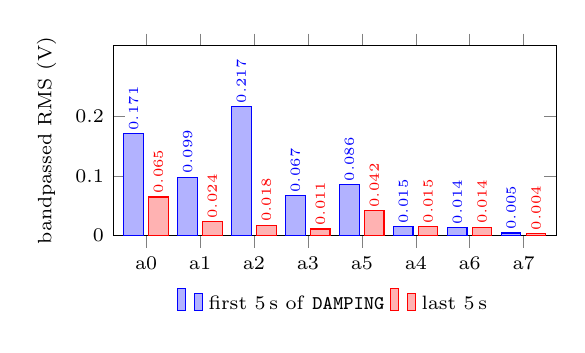
\begin{tikzpicture}
        \begin{axis}[width=7.2cm, height=4.0cm, ybar, bar width=7pt,
                     xtick={1,2,3,4,5,6,7,8},
                     xticklabels={a0,a1,a2,a3,a5,a4,a6,a7},
                     xmin=0.4, xmax=8.6, ymin=0, ymax=0.32,
                     ytick={0,0.1,0.2},
                     ylabel={bandpassed RMS (V)},
                     legend style={at={(0.5,-0.24)}, anchor=north,
                                   legend columns=2, draw=none, fill=none},
                     nodes near coords={\pgfmathprintnumber[fixed,zerofill,precision=3]{\pgfplotspointmeta}},
                     every node near coord/.append style={font=\tiny, rotate=90,
                                                          anchor=west, inner sep=1pt}]
          \addplot coordinates {(1,0.1714) (2,0.0986) (3,0.2171) (4,0.0672)
                                (5,0.0860) (6,0.0149) (7,0.0140) (8,0.0046)};
          \addlegendentry{first 5\,s of \texttt{DAMPING}}
          \addplot coordinates {(1,0.0651) (2,0.0235) (3,0.0179) (4,0.0113)
                                (5,0.0420) (6,0.0152) (7,0.0144) (8,0.0040)};
          \addlegendentry{last 5\,s}
        \end{axis}
      \end{tikzpicture}\\
      {\scriptsize 40\,s of damping, eight channels.}
    \end{column}
    \begin{column}{0.44\textwidth}
      \scriptsize\raggedright
      \texttt{STEADY\_GAIN[5]} $= -0.015$ was a \textbf{prediction}: a5's DC
      diagonal is $-7$\,counts/V against a block mean of \textbf{4}, under
      $2\times$ the noise. A wrong sign \emph{pumps}.

      \vspace{1.5mm}
      \textbf{It damped: $0.0860 \to 0.0420$\,V}, while ch0 fell
      $0.1714 \to 0.0651$.

      \vspace{1.5mm}
      \textbf{The three at zero gain are the control.} a4/a6/a7 are
      \textbf{flat to three decimals} across 40\,s that took a factor of
      \textbf{3--12} out of every real channel.

      \vspace{1.5mm}
      \textbf{Then the newer measurement retracted it.} The
      fixed-frequency refit (2026-08-06) finds a5's residue \textbf{not
      distinguishable from its own noise}, and a gain on a channel that measures
      noise \emph{injects} actuator noise while damping nothing.

      \vspace{1.5mm}
      \textbf{\texttt{delta} ships \texttt{STEADY\_GAIN[5]} $= 0$.} The two measurements
      disagree and \textbf{the one with error bars wins}. a5 is still in the
      quorum while nothing drives it, which is what holds the rig out of
      \texttt{LOCKED}.
    \end{column}
  \end{columns}
\end{frame}
\note{The other half of the eight-channel result, and it has a second act I like
even more than the first.

a5's gain was set to minus 0.015 before anyone knew whether a5 worked. The only
evidence for the sign was a5's own diagonal in the DC actuation matrix, minus
seven counts per volt in a block whose mean absolute response is four. Under two
times the noise. And the failure mode is not "it does nothing": a wrong-signed
channel pumps its mode.

It damped. Over forty seconds a5's bandpassed RMS went from 0.0860 volts to
0.0420, while channel zero went from 0.1714 to 0.0651 alongside it.

The control group is in the same chart. a4, a6 and a7 shipped at zero gain and
are flat to three decimal places across forty seconds that took a factor of three
to twelve out of every real channel.

Now the second act. A fixed-frequency refit of the eight-coil dither run on the
same day finds a5's residue not distinguishable from its own noise. A gain on a
channel that measures noise injects actuator noise while damping nothing. So delta
drops a5 to zero gain. Two measurements disagree, and the one with error bars
wins. That is the rule I would want people to take from this slide, not the
happy first result.

And a5 staying in the quorum while being driven by nothing is exactly the bug
that stops the rig announcing LOCKED. That is slide 50.}

% ================================================================ 42
\begin{frame}{\texttt{delta}: eight channels, and the wire stops throttling the loop}
  \footnotesize
  \begin{columns}[T]
    \begin{column}{0.52\textwidth}
      \textbf{1. \texttt{sat-window}: a bug fix, not a retune.}
      \texttt{MAX\_CONSECUTIVE\_SATURATED = 30} counted \emph{samples}, so it
      meant 0.41 / 1.28 / 1.65 / \textbf{2.40}\,s at 1 / 4 / 5 / 8 coils, and
      one clean sample erased the whole streak.

      \vspace{1mm}
      Now \texttt{SAT\_SUSTAIN\_S} $= 1.30$\,s with \texttt{SAT\_FRACTION}
      $= 0.80$: the shape the \emph{rail} check has always had.
      $30 \times 42.6$\,ms $= \mathbf{1.278}$\,s, so it is
      \textbf{behaviour-preserving on four channels}.

      \vspace{1mm}
      It goes \textbf{first}, because the other two changes both move the sample
      rate. \emph{You do not move a sample rate underneath a sample-counted
      threshold.}

      \vspace{2mm}
      \textbf{2. \texttt{fast-transport}.} \texttt{pyDAC2.FastDAC} writes and
      returns with no ack wait, and the baud goes $115200 \to 500000$.
      \textbf{18\,Hz $\to$ 1111\,Hz.} Requires a reflash; a host at the
      wrong baud fails preflight with ``never sent \texttt{READY}''.
    \end{column}
    \begin{column}{0.46\textwidth}
      \textbf{3. All eight enabled}, with a4/a6/a7 as \emph{sensors} at
      \textbf{zero gain}.

      \vspace{1mm}
      \textbf{\texttt{baseline-floor} demotes all three on the first
      calibration, and that is the designed outcome.} \texttt{ENABLE\_CHANNEL}
      stops being a constant somebody maintains and becomes \textbf{a
      measurement the rig makes every time it calibrates}.

      \vspace{2mm}
      \textbf{And then it damped worse than everything before it.}

      \vspace{1mm}
      \centering
      {\scriptsize\setlength{\tabcolsep}{3.5pt}
      \begin{tabular}{@{}lccc@{}}
        \toprule
        240\,s, 3 kicks & DAMPING & FAULT & faults \\
        \midrule
        \texttt{beta} (4ch, 23\,Hz) & \textbf{83.1\%} & 8.5\% & 4 \\
        the eight-channel step (8ch, 18\,Hz) & 74.1\% & 15.0\% & 8 \\
        the 500000-baud step (8ch, 1111\,Hz) & \textbf{42.3\%} &
          25.3\% & 11 \\
        \bottomrule
      \end{tabular}}

      \vspace{1.5mm}
      \raggedright
      \alert{\textbf{A 49$\times$ faster wire made the damping worse.}}
    \end{column}
  \end{columns}
\end{frame}
\note{the 500000-baud step is three changes about one thing: an eight-channel rig runs a loop a
four-channel rig does not. No gain and no threshold is retuned.

sat-window first, and the ordering matters. Max consecutive saturated counted
iterations, and both halves of that were wrong. Samples are not seconds, so
thirty samples meant 0.41 seconds on one coil and 2.40 on eight, and the interlock
got less sensitive precisely as the rig got harder to control. And "consecutive"
meant one clean sample of ADC noise erased all the accumulated evidence. The fix
is the shape the rail check has always had. The number is chosen so that thirty
iterations times the measured four-coil period comes to 1.278 seconds, so 1.30 is
behaviour-preserving on four channels. That is what makes it a bug fix rather
than a retune, and it is why it goes first.

Second, fast-transport. The ack wait goes away and the baud goes to 500000. 18
hertz to 1111. Giving up the ack is safe for a boring reason: ERR comes back for
exactly two things, a malformed command and a bad channel number, FastDAC rejects
both locally, and no controller has ever branched on an OK.

Third, all eight enabled with a4, a6 and a7 at zero gain, letting baseline-floor
demote them every calibration.

And then the result. the 500000-baud step damped 42.3 percent of the run against beta's 83.1 and
the eight-channel step's 74.1, with eleven faults. A forty-nine-fold faster wire made the damping
worse. That is the setup for the two best defect slides in the deck.}

% ================================================================ 43
\begin{frame}{Defect 7: a torn serial frame, and 45\,V into a 0.5\,V rail}
  \begin{columns}[T]
    \begin{column}{0.49\textwidth}
      \footnotesize
      \rawdata\ \texttt{read\_sample()} accepts any row whose first character is
      a digit and which splits into $\geq N$ fields.

      \vspace{1mm}
      \centering
      {\scriptsize\ttfamily
      \begin{tabular}{@{}l@{}}
        \toprule
        \rm valid, every field in 0..1023 \\
        612,634,701,688,559,548,861,733 \\
        \midrule
        \rm torn: 8 fields, first char a digit, \rm accepted \\
        612,634,522676,688,559,548,861,733 \\
        \bottomrule
      \end{tabular}}

      \vspace{2mm}
      \raggedright
      \textbf{Where it comes from.} \texttt{fast-transport} stopped draining the
      board's \texttt{OK ch=.. v=..} ack, so acks now interleave with data rows
      and a buffer boundary splices two fields' digits together.

      \vspace{2mm}
      \alert{\textbf{The speed-up created the defect.}} the 500000-baud step's own 240\,s log
      carries \textbf{ten} rows with a count outside 0..1023 (5659, 65690,
      522676). \textbf{Zero} such rows appear in any of the \textbf{four} slower
      logs from the same session.
    \end{column}
    \begin{column}{0.49\textwidth}
      \footnotesize
      \goeswrong\ Follow one sample through the loop:

      \vspace{1mm}
      \centering
      {\scriptsize
      \begin{tabular}{@{}rll@{}}
        \toprule
        & value & step \\
        \midrule
        1 & $522676$ counts & the torn field \\
        2 & $\times\,5.02/1023$ & $= 2564.8$\,V raw \\
        3 & $\times\,\alpha_{\mathrm{LP}} = 0.0178$ &
            $= \mathbf{+45.6}$\,\textbf{V} into bp \\
        4 & rings down, $\tau_{\mathrm{HP}} = 0.398$\,s & the 0.4\,Hz highpass \\
        5 & $\hat{v}$ peaks & $= \mathbf{1401}$\,\textbf{V/s} \\
        6 & $P = 0.030 \times 1401$ &
            $= \mathbf{42}$\,\textbf{V demanded} \\
        \midrule
        & rail & $\mathbf{0.5}$\,\textbf{V} \\
        \bottomrule
      \end{tabular}}

      \vspace{1mm}
      {\scriptsize $\alpha_{\mathrm{LP}} = \Delta t / (\Delta t +
      \tfrac{1}{2\pi \cdot 3\,\mathrm{Hz}})$ at $\Delta t = 0.96$\,ms.}

      \vspace{2mm}
      \raggedright
      One bad character pins the actuator for the whole 0.4\,s ringdown of the
      highpass. \textbf{Four of the 500000-baud step's twelve entries to \texttt{FAULT}
      follow a torn line within 2\,s}, and the first starts the
      4\,s-\texttt{DAMPING} / 5\,s-\texttt{FAULT} thrash that eats the middle of
      the run.
    \end{column}
  \end{columns}
\end{frame}
\note{The defect that explains why a forty-nine times faster wire damped worse.

read_sample accepted any row whose first character is a digit and which splits
into at least N fields. That is a shape check, not a value check, and the torn
row on the slide passes it: eight fields, first character a digit, one of them
five hundred and twenty-two thousand.

It was harmless while the acknowledgement was being drained. fast-transport
stopped draining it, so the board's OK replies now arrive interleaved with data
rows, and a buffer boundary splices two fields' digits together.

The evidence that the speed-up created the defect is on the left. Ten such rows
in the 500000-baud step's own 240 second log, and zero in any of the four slower logs from the
same session.

The right column is the cost of one of them, and it is worth reading out. 522676
counts times 5.02 volts over 1023 counts is 2565 volts of raw scale. A single
sample through the 3 hertz lowpass keeps about one part in fifty-six of that, so
45.6 volts lands in the bandpass. That then rings down over the 0.4 hertz
highpass with a time constant of 0.398 seconds, so it is not one bad sample, it
is four hundred milliseconds of corrupted signal. The velocity estimate peaks at
1401 volts per second, and P times that is 42 volts demanded into a rail of half
a volt.

Four of the 500000-baud step's twelve entries to FAULT follow a torn line within two seconds, and
the first one starts the thrash that eats the middle of the run.}

% ================================================================ 44
\begin{frame}{\texttt{sample-guard} and \texttt{decimate}, and why they ship together}
  \begin{columns}[T]
    \begin{column}{0.49\textwidth}
      \footnotesize
      \thefix\ \texttt{sample-guard}: a count outside
      \texttt{0..ADC\_MAX\_COUNTS} is a \textbf{framing error}, dropped exactly
      the way an \texttt{OK} line is. Three lines.

      \vspace{1.5mm}
      Replayed offline over the same the 500000-baud step log, ch0's velocity estimate:

      \vspace{1mm}
      \centering
      {\scriptsize
      \begin{tabular}{@{}lrr@{}}
        \toprule
        ch0 velocity & the 500000-baud step & \textbf{+guard} \\
        \midrule
        rms (V/s) & 13.109 & \textbf{5.413} \\
        peak (V/s) & 1441 & \textbf{41} \\
        \bottomrule
      \end{tabular}}

      \vspace{1.5mm}
      \raggedright
      \textbf{A 35$\times$ reduction in peak, on data already recorded.} No
      bench time, no hardware change.
    \end{column}
    \begin{column}{0.49\textwidth}
      \footnotesize
      \textbf{\texttt{decimate}: give the loop its own clock.} Read the wire at
      full rate; run the control step at \texttt{CONTROL\_HZ} $= 100$ on the
      \emph{mean} of whatever arrived since the last one.

      \vspace{1mm}
      \textbf{Why:} the arrival rate has been $24 / 12.5 / 18 / 1111$\,Hz, and
      every gain, filter and interlock here was tuned against one of them.

      \vspace{2mm}
      \centering
      {\scriptsize
      \begin{tabular}{@{}lrr@{}}
        \toprule
        ch0 velocity rms (V/s) & \textbf{with} guard & \textbf{without} \\
        \midrule
        the 500000-baud step & 13.109 & 13.109 \\
        $+$ decimate & \textbf{4.732} & \textbf{23.4} \\
        \bottomrule
      \end{tabular}}

      \vspace{1.5mm}
      \raggedright
      \alert{\textbf{Without the guard, decimation makes it worse.}} A boxcar
      mean \emph{spreads} one bad sample across a whole step instead of
      confining it to one. \textbf{The two are not separable.}

      \vspace{1.5mm}
      {\scriptsize Phase cost is measured: 100\,Hz gives back 13.1$^\circ$ at
      3.75\,Hz against the 500000-baud step's wire, and still holds 18.4$^\circ$ \emph{more} than
      the four-coil configuration every gain here was validated at.}
    \end{column}
  \end{columns}
\end{frame}
\note{Two fixes, and the reason they cannot be separated.

sample-guard is three lines: a count outside the ADC range is a framing error and
is dropped like an OK line. Replayed offline over the same the 500000-baud step log, ch0's
velocity estimate goes from 13.1 to 5.4 volts per second rms, and the peak from
1441 to 41. A thirty-five fold reduction in peak, recovered from data already on
disk with no bench time at all.

decimate gives the loop its own clock. Read the wire at whatever rate it runs and
take a control step at a fixed 100 hertz on the mean of whatever arrived. The
justification is that the arrival rate moved four times in three days, from 24 to
12.5 to 18 to 1111 hertz, and every gain, filter and interlock in the file was
tuned against one of those numbers. A control rate the file owns is a rate that
stops moving underneath them.

Now the interaction, which is the interesting part. With the guard, decimation
takes rms from 5.4 to 4.7. Without the guard it takes it from 13.1 to 23.4, which
is worse than doing nothing, because a boxcar mean spreads one bad sample across
a whole control step instead of confining it to one sample. That is why the two
ship together and why the guard goes first.

And the phase cost was measured rather than assumed. 100 hertz gives back 13.1
degrees at 3.75 hertz against the 500000-baud step's raw wire, and still holds 18.4 degrees more
margin than the four-coil configuration in which every gain in the file was
originally validated.}

% ================================================================ 45
\begin{frame}{Defect 8: the runaway breaker was reading the \emph{beat}}
  \begin{columns}[T]
    \begin{column}{0.46\textwidth}
      \footnotesize
      \rawdata\ Three modes, measured to \textbf{0.0005\,Hz} on the 320\,s quiet
      record. Beat period $= 1/|f_i - f_j|$:

      \vspace{1mm}
      \centering
      {\scriptsize
      \begin{tabular}{@{}lcc@{}}
        \toprule
        pair & $|\Delta f|$ (Hz) & beat period \\
        \midrule
        A--B & 0.2794 & \textbf{3.578\,s} \\
        B--C & 0.6447 & \textbf{1.551\,s} \\
        A--C & 0.9241 & \textbf{1.082\,s} \\
        \bottomrule
      \end{tabular}}

      \vspace{1mm}
      {\scriptsize $f_A = 0.7155$, $f_B = 0.9949$, $f_C = 1.6396$\,Hz.}

      \vspace{2mm}
      \raggedright
      \texttt{RUNAWAY\_TREND\_LAG\_S = 2.0} sits inside all three. It
      was chosen in \texttt{beta}, before any of these frequencies was known.

      \vspace{2mm}
      \goeswrong\ $\mathrm{env}(t)$ and $\mathrm{env}(t-2\mathrm{s})$ land on
      \emph{different phases of the beat}. The test measures the beat and calls
      it growth.
    \end{column}
    \begin{column}{0.52\textwidth}
      \centering
      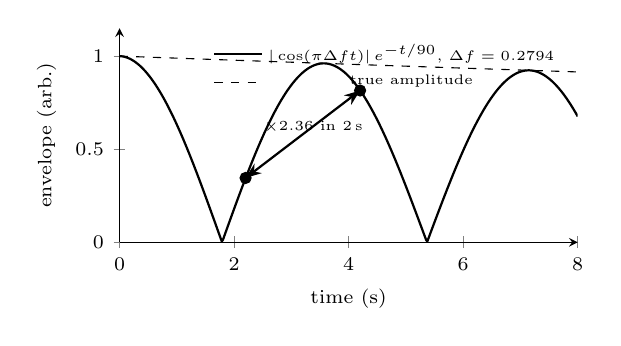
\begin{tikzpicture}
        \begin{axis}[width=7.4cm, height=4.3cm,
                     xlabel={time (s)}, ylabel={envelope (arb.)},
                     xmin=0, xmax=8, ymin=0, ymax=1.15,
                     axis lines=left, xtick={0,2,4,6,8},
                     legend style={at={(0.98,0.98)}, anchor=north east,
                                   draw=none, fill=none, font=\tiny}]
          \addplot[thick, domain=0:8, samples=400]
            {abs(cos(deg(0.8778*x)))*exp(-x/90)};
          \addlegendentry{$|\cos(\pi\Delta f t)|\,e^{-t/90}$, $\Delta f = 0.2794$}
          \addplot[dashed, domain=0:8, samples=60] {exp(-x/90)};
          \addlegendentry{true amplitude}
          \addplot[only marks, mark=*, mark size=2pt]
            coordinates {(2.2,0.3455) (4.2,0.8154)};
          \draw[{Stealth[length=2mm]}-{Stealth[length=2mm]}, thick]
            (axis cs:2.2,0.3455) -- (axis cs:4.2,0.8154);
          \node[font=\tiny, anchor=west] at (axis cs:2.35,0.62)
            {$\times 2.36$ in 2\,s};
        \end{axis}
      \end{tikzpicture}\\
      {\scriptsize Toy model, the A--B pair. At $t = 2.2$\,s the envelope reads
      \textbf{0.3455}; at $t = 4.2$\,s it reads \textbf{0.8154}. The test asks
      for $>1.02\times$ and gets \textbf{2.36}$\times$, while the \emph{true}
      amplitude has \emph{fallen} \textbf{2.2\%}.}
    \end{column}
  \end{columns}
\end{frame}
\note{The defect that made delta damp, and it is my favourite in the deck because
the mechanism is arithmetic you can do on a napkin.

The runaway growth test compares the envelope now against the envelope one lag
ago and faults if it grew by more than two percent. The lag was set to two
seconds in beta, before anyone had measured the mode frequencies.

The frequencies are now known to half a millihertz: 0.7155, 0.9949 and 1.6396
hertz. Three modes beating against each other give beat periods of 3.578, 1.551
and 1.082 seconds. A two-second lag sits inside all three, which means the
envelope now and the envelope two seconds ago land on different phases of the
beat.

The plot is the toy model, using the A-B pair only. The solid line is the beating
envelope of two equal sines 0.2794 hertz apart, multiplied by a real ninety
second decay. The dashed line is the true amplitude. Sample it at 2.2 seconds and
you read 0.3455. Sample it two seconds later at 4.2 and you read 0.8154. That is
a factor of 2.36, against a threshold of 1.02, so the breaker faults, while the
true amplitude has fallen by two point two percent over the same interval.

The optic was being damped. The supervisor was watching a beat.}

% ================================================================ 46
\begin{frame}{Defect 8, other half: a real ringdown was invisible too}
  \begin{columns}[T]
    \begin{column}{0.48\textwidth}
      \footnotesize
      \rawdata\ $\tau_{\mathrm{env}}$, the decay of the \emph{envelope the
      breaker watches} after a kick, measures \textbf{56--130\,s}. How far does
      that fall in one lag?

      \vspace{1mm}
      \centering
      {\scriptsize
      \begin{tabular}{@{}lcc@{}}
        \toprule
        & $\tau_{\mathrm{env}} = 56$\,s & $130$\,s \\
        \midrule
        fall in \textbf{2\,s} & 3.5\% & \textbf{1.5\%} \\
        fall in \textbf{10\,s} & \textbf{16.4\%} & \textbf{7.4\%} \\
        \midrule
        \multicolumn{3}{@{}l}{threshold: 2\%} \\
        \bottomrule
      \end{tabular}}

      \vspace{1.5mm}
      \raggedright
      \goeswrong\ At \texttt{LAG} $= 2$\,s a genuine ringdown moves
      \textbf{1.5--3.6\%}, straddling the 2\% line. The breaker could not
      tell a real decay from a beat, in either direction.

      \vspace{1.5mm}
      \thefix\ \texttt{RUNAWAY\_TREND\_LAG\_S} $2.0 \to \mathbf{10.0}$\,s:
      \textbf{2.8$\times$} the longest beat, \textbf{5.6--13$\times$} shorter
      than $\tau_{\mathrm{env}}$.

      \vspace{1.5mm}
      \textbf{The remaining 14.4\% is not thrash.} $7 \times 5$\,s of mandatory
      hold $= 35$\,s $= 14.3\%$ of 244.5\,s.
    \end{column}
    \begin{column}{0.50\textwidth}
      \centering
      {\scriptsize
      \begin{tabular}{@{}lcccc@{}}
        \toprule
        \% of time & DAMP & FAULT & CALIB & entries \\
        \midrule
        \texttt{LAG} $= 2.0$ & 54.1 & 25.2 & 20.7 & 10 \\
        \textbf{\texttt{LAG} $= 10.0$} & \textbf{77.5} & \textbf{14.4} &
          \textbf{8.2} & \textbf{7} \\
        \midrule
        \multicolumn{5}{@{}l}{\emph{whole suite, everything else identical}} \\
        \texttt{LAG} $= 2.0$ & \multicolumn{4}{l}{43 passed / 7 failed} \\
        \textbf{\texttt{LAG} $= 10.0$} & \multicolumn{4}{l}{42 passed /
          8 failed} \\
        \bottomrule
      \end{tabular}}\\[1mm]
      {\scriptsize Two runs, 244.5\,s, five hand kicks.}

      \vspace{2mm}
      \raggedright\footnotesize
      \alert{\textbf{The fix is not free.}} \textbf{One assertion flips: the
      wrong-sign detector.} With ch2 inverted over 120\,s, a 2\,s lag trips the
      breaker \textbf{$\geq$3} times and a 10\,s lag trips it \textbf{2}. The
      check demands 3.

      \vspace{1mm}
      \textbf{The wrong sign is still caught}: the companion
      \texttt{faults > 0} passes at both. A breaker that no longer reads a
      1.55\,s beat as growth also fires less often on something genuinely
      growing.

      \vspace{1.5mm}
      \textbf{Not a win over \texttt{beta}'s 83.1\%}: different kick schedule.
    \end{column}
  \end{columns}
\end{frame}
\note{The other half of the same defect, and it is the half that shows the test
was broken in both directions.

Ask what a genuine ringdown does over one lag. The measured closed-loop decay
constant is 56 to 130 seconds. Over two seconds that is a fall of 1.5 to 3.6
percent, straddling the two percent threshold the test uses. So the breaker could
not reliably see a real decay either. It was not that the test was too sensitive;
it was that at a two-second lag there was almost no signal in it at all.

The fix is one constant, and the two tables on the right are the result, measured
back to back on the same evening with the same gains.

The remaining fault time is accounted for exactly: seven entries times the
five-second mandatory hold is 35 seconds against the 14.4 percent measured. It is
the hold, not the breaker re-tripping.

Now the honest cost, and I want it said rather than skipped. Run the whole suite
at each lag value with everything else identical and the score goes from 43
passed and 7 failed at two seconds to 42 passed and 8 failed at ten. Exactly one
assertion flips, and it is the wrong-sign detector: with channel two's gain
deliberately inverted over a 120 second run, a two-second lag trips the breaker
three or more times and a ten-second lag trips it twice, against a check that
demands three. The wrong sign is still caught, because the companion assertion
that faults are non-zero passes at both values. But the trade is real: a breaker
that no longer reads a 1.55 second beat as growth also fires less often on
something that genuinely is growing.

The last box is the discipline point and I want it said out loud. Do not put
77.5 next to beta's 83.1 and call it a win or a loss. beta's three kicks were
scripted; delta's five were by hand at unrecorded strength and hard enough to clip
every channel. The comparisons that are controlled are delta against the 500000-baud step and delta
against itself across the lag change, and both are on this slide.}

% ================================================================ 47
\begin{frame}{Defect 9: stationarity is not quietness}
  \begin{columns}[T]
    \begin{column}{0.50\textwidth}
      \footnotesize
      \rawdata\ Caught on hardware: a fresh calibration produced a noise floor
      \textbf{11.5$\times$} the trusted one.

      \vspace{1mm}
      What that does to every derived threshold, taking \texttt{alpha}'s ch0 floor as the
      trusted value:

      \vspace{1mm}
      \centering
      {\scriptsize
      \begin{tabular}{@{}lcc@{}}
        \toprule
        & trusted & inflated $11.5\times$ \\
        \midrule
        baseline (V) & 0.1804 & 2.075 \\
        runaway line, $1.8\times$ & 0.325 & 3.735 \\
        lock line, $0.35\times$ & 0.063 & 0.726 \\
        \bottomrule
      \end{tabular}}

      \vspace{2mm}
      \raggedright
      \goeswrong\ The breaker goes blind and the rig declares \texttt{LOCKED} at
      \textbf{11.5$\times$} the residual motion it should require. The
      calibration measured the \emph{ringing}, not the room.

      \vspace{1mm}
      And \texttt{persist-baseline} would carry it across restarts.
    \end{column}
    \begin{column}{0.48\textwidth}
      \footnotesize
      \thefix\ \texttt{baseline-sanity}. A fresh floor that fails the check is
      \textbf{refused} and the trusted one kept. On the bench the 11.5$\times$
      floor was refused.

      \vspace{2mm}
      \textbf{And the guard needs a guard.}
      \texttt{MAX\_BASELINE\_REFUSALS = 3} stops it refusing forever if the room
      genuinely \emph{did} get louder.

      \vspace{2.5mm}
      \textbf{What the persistence buys.} The noise floor is a property of the
      room, not of the run, so \texttt{delta} writes it to disk and reuses it across
      restarts, behind a config fingerprint, an age limit and a sanity check.

      \vspace{1mm}
      \centering
      {\footnotesize
      \begin{tabular}{@{}lcc@{}}
        \toprule
        cold-start calibration & before & \textbf{after} \\
        \midrule
        & 20\,s & \textbf{2.0\,s} \\
        \bottomrule
      \end{tabular}}

      \vspace{1.5mm}
      \raggedright
      {\scriptsize This completes defect 3, nine versions later. \texttt{alpha} made one bad
      sub-window outvotable; \texttt{delta} makes a bad \emph{whole calibration} refusable.}
    \end{column}
  \end{columns}
\end{frame}
\note{Defect nine closes the loop opened by defect three, nine versions earlier.

The noise floor is measured during CALIBRATING with the gain at zero. The
assumption is that a window with the gain off is a window of room noise. It is
not. Stationarity is not quietness: a calibration taken while the optic is still
ringing measures the ringing.

This was caught on hardware. A fresh calibration produced a floor 11.5 times the
trusted one. The left column is what that costs, using alpha's channel zero floor as
the trusted number. The runaway trip line goes from 0.325 volts to 3.7, so the
breaker is effectively blind, and the lock line goes from 0.063 to 0.726, so the
rig would announce LOCKED at 11.5 times the residual motion it should demand.

And persist-baseline makes it worse, because a bad floor would now survive across
process restarts.

So baseline-sanity refuses a fresh floor that fails the check and keeps the
trusted one. On the bench that 11.5 times floor was refused.

The guard needs a guard, which is the part I like. Max baseline refusals is
three, so if the room genuinely did get louder the controller cannot sit there
refusing reality forever.

The persistence itself is what takes cold-start calibration from twenty seconds
to two, and twenty seconds of zero gain was the single biggest waste the build before beta went
after.}

% ================================================================ PART V
\section{Open defects}

% ================================================================ 48
\begin{frame}{Open defect 1: the rig locks, and cannot say so}
  \begin{columns}[T]
    \begin{column}{0.52\textwidth}
      \footnotesize
      \rawdata\ \textbf{Zero} \texttt{*** LOCKED ***} lines in \emph{every} run
      of the 2026-08-06 session: the eight-channel step, the 500000-baud step and \texttt{delta} have never printed it. The
      lock time is \textbf{the deliverable}.

      \vspace{1.5mm}
      \textbf{But the rig does lock.} The four \texttt{ch\{i\}\_locked} columns
      are simultaneously 1 for \textbf{6 distinct episodes} on the good \texttt{delta} run,
      and \textbf{3} on the run before it.

      \vspace{2mm}
      \goeswrong\ The announcement needs
      \texttt{self.locked[live].all()}, where
      \texttt{live = enabled \& healthy} and \texttt{ENABLE\_CHANNEL} is
      \texttt{True} on \emph{all eight}.

      \vspace{1.5mm}
      \alert{\textbf{One undriven channel vetoes the whole rig, permanently.}}
      This is a quorum bug, not a damping failure.
    \end{column}
    \begin{column}{0.46\textwidth}
      \centering
      {\scriptsize
      \begin{tabular}{@{}lcccc@{}}
        \toprule
        & in \texttt{live}? & driven? & ratio & \texttt{locked} \\
        \midrule
        a0 & yes & yes & $<0.35$ & 1 \\
        a1 & yes & yes & $<0.35$ & 1 \\
        a2 & yes & yes & $<0.35$ & 1 \\
        a3 & yes & yes & $<0.35$ & 1 \\
        \midrule
        \textbf{a5} & \textbf{yes} & \textbf{no} &
          \textbf{1.26--2.53} & \textbf{0} \\
        \midrule
        a4 & no (\texttt{NOSIG}) & no & n/a & n/a \\
        a6 & no (\texttt{NOSIG}) & no & n/a & n/a \\
        a7 & no (\texttt{NOSIG}) & no & n/a & n/a \\
        \bottomrule
      \end{tabular}}

      \vspace{1.5mm}
      \raggedright\footnotesize
      a4, a6 and a7 demote themselves to \texttt{NOSIG} and leave \texttt{live}.
      \textbf{a5 does not}: it stays healthy, so it is in the quorum, but
      \texttt{STEADY\_GAIN[5]} $= 0$ so nothing drives it.

      \vspace{1.5mm}
      \thefix\ \textbf{Not yet applied.} Drop zero-gain channels from
      the quorum. \textbf{One line}, and first on the open list.
    \end{column}
  \end{columns}
\end{frame}
\note{The open defect that matters most, because the lock time is the stated
deliverable and we have not produced one since 2026-08-04.

Zero LOCKED lines in every run of the 08-06 session. the eight-channel step, the 500000-baud step and delta have never
printed it.

The first thing to establish is that this is not a damping failure. The CSV
carries a per-channel locked flag, and on the good delta run the four real channels
are simultaneously locked for six distinct episodes. The rig locks. It just
cannot say so.

The table is the cause. The announcement requires every live channel to be
locked, where live means enabled and healthy, and ENABLE_CHANNEL is true on all
eight. a4, a6 and a7 demote themselves to NOSIG, so they drop out of live. a5
does not: it stays healthy, so it stays in the quorum. But delta ships a5 at zero
gain, for the good reason on the a5 slide, so nothing drives it, and it sits at
a ratio between 1.26 and 2.53 against a lock line of 0.35.

One undriven channel vetoes the whole rig, permanently.

The fix is one line: drop zero-gain channels from the quorum, or set
ENABLE_CHANNEL false on a5. It is not applied yet, and it is first on the open
list.}

% ================================================================ 49
\begin{frame}{Open defect 2: no OSEM rests at mid-scale}
  \footnotesize
  The ADC reads \textbf{0 to 1023 counts}, so \textbf{mid-scale is 511.5}. Room
  before a rail is \textbf{above} $= 1023 -$ resting, \textbf{below} $=$ resting.

  \vspace{1mm}
  \begin{columns}[T]
    \begin{column}{0.49\textwidth}
      \rawdata\ Resting counts, \texttt{CALIBRATING}, 22\,246 samples, outputs
      at bias:

      \vspace{1mm}
      \centering
      {\scriptsize\setlength{\tabcolsep}{4pt}
      \begin{tabular}{@{}lcccc@{}}
        \toprule
        & ch0 & ch1 & \textbf{ch2} & ch3 \\
        \midrule
        resting count & 601.2 & 630.3 & \textbf{686.5} & 681.8 \\
        room above & 422 & 393 & \textbf{336} & 341 \\
        room below & 601 & 630 & \textbf{686} & 682 \\
        \bottomrule
      \end{tabular}}

      \vspace{1.5mm}
      \raggedright
      \textbf{Every channel rests \emph{above} mid-scale, so every channel meets
      its \emph{top} rail first.} ch2 is worst, with \textbf{2.0$\times$} as much
      room below as above.
    \end{column}
    \begin{column}{0.48\textwidth}
      \goeswrong\ \textbf{A railed sensor is outside its linear region}, so the
      velocity estimate from it is wrong exactly when the optic is moving
      hardest and the loop is pushing hardest.

      \vspace{1.5mm}
      \centering
      {\scriptsize\setlength{\tabcolsep}{4pt}
      \begin{tabular}{@{}lcccc@{}}
        \toprule
        of 251\,280 samples & ch0 & ch1 & \textbf{ch2} & ch3 \\
        \midrule
        railed & 2.9\% & 0.8\% & \textbf{3.6\%} & 0.9\% \\
        \texttt{rail} interlock caught & 136 & 0 & 51 & 0 \\
        \bottomrule
      \end{tabular}}

      \vspace{1.5mm}
      \raggedright
      The interlock needs the pin \emph{sustained}, so it caught \textbf{187} of
      \textbf{20{,}696}. \alert{\textbf{About 99\% of this clipping is invisible
      to every interlock.}}
    \end{column}
  \end{columns}

  \vspace{2mm}
  {\footnotesize \thefix\ \textbf{Proposed, not yet run: the bias
  sweep.} Coil bias is a static force, so step one channel $0.10 \to 0.40$\,V at
  zero gain and log the resting counts. \textbf{If they move}, the offset is
  electromagnetic and a bias trim removes it; \textbf{if not}, it is mechanical
  flag alignment. \textbf{Two commands and a log.}}
\end{frame}
\note{The open hardware defect underneath every number in this deck, and it
starts from the sensor geometry.

Every channel rests above mid-scale, so every one meets its top rail first, and
channel two is worst at a factor of two.

Now the consequence, which is the point of the slide. A railed sensor is outside
its linear region. So the velocity estimate derived from it is wrong exactly when
the optic is moving hardest and the loop is pushing hardest. That is the worst
possible moment for the measurement to fail.

And it is nearly invisible. Between 0.8 and 3.6 percent of samples on each
channel are at or beyond a rail, twenty thousand of them in total, and the rail
interlock caught 187, because it requires the pin to be sustained and this
clipping is transient. About ninety-nine percent of it never becomes a fault.

The proposed fix costs no code. Coil bias is a static force, so step one channel
from 0.10 to 0.40 volts with the gain at zero and log the resting counts. If they
move, the offset is electromagnetic and a per-channel bias trim removes it at
source. If they do not move, it is mechanical flag alignment. Either answer is
worth having.}

% ================================================================ 50
\begin{frame}{Open defect 3: the clipping is arithmetic, not bad luck}
  \centering
  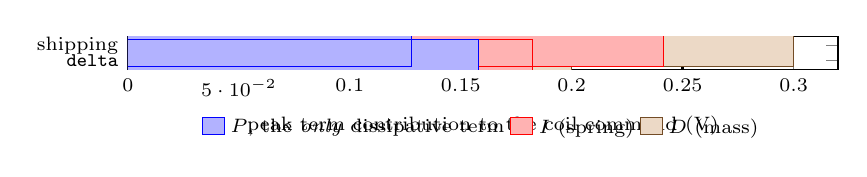
\begin{tikzpicture}
    \begin{axis}[width=10.6cm, height=2.0cm, xbar stacked, bar width=15pt,
                 xmin=0, xmax=0.32, ymin=-0.6, ymax=1.6,
                 ytick={0,1}, yticklabels={\textbf{\texttt{delta}}, shipping},
                 y tick label style={font=\scriptsize},
                 xlabel={peak term contribution to the coil command (V)},
                 xtick={0,0.05,0.10,0.15,0.20,0.25,0.30},
                 legend style={at={(0.5,-1.15)}, anchor=north,
                               legend columns=3, draw=none, fill=none}]
      \addplot coordinates {(0.1279,1) (0.1580,0)};
      \addlegendentry{$P$, the \emph{only} dissipative term}
      \addplot coordinates {(0.1135,1) (0.0243,0)};
      \addlegendentry{$I$ (spring)}
      \addplot coordinates {(0.0584,1) (0.0178,0)};
      \addlegendentry{$D$ (mass)}
      \draw[dashed, very thick] (axis cs:0.25,-0.6) -- (axis cs:0.25,1.6);
      \node[font=\tiny, anchor=south west] at (axis cs:0.252,1.15)
        {\texttt{VMAX}$-$\texttt{BIAS} $= 0.25$\,V};
    \end{axis}
  \end{tikzpicture}

  \vspace{7mm}
  \begin{columns}[T]
    \begin{column}{0.48\textwidth}
      \footnotesize\raggedright
      \rawdata\ Shipping gains, peak demand:
      \[ 0.1279 + 0.1135 + 0.0584 = \mathbf{0.2998}\ \mathrm{V} \]
      against a half-window of \textbf{0.250\,V}. \alert{\textbf{120\% of
      budget.}}

      \vspace{1mm}
      \goeswrong\ \textbf{The channels clip because the demand exceeds the
      window, not because of bad luck.} And the largest item, \textbf{$K_i$ at
      0.1135\,V, 38\%}, dissipates \emph{nothing}: the integrator sits behind
      the 0.4\,Hz highpass, so $i = -K_i\,\mathrm{bp}$ and bp carries no DC to
      reject.
    \end{column}
    \begin{column}{0.48\textwidth}
      \footnotesize\raggedright
      Nothing in this project justifies \texttt{KI\_GAIN} or
      \texttt{KD\_GAIN}. Not a scope trace, not a sweep, not a sentence.
      $-0.030$ has one. And the early four-channel build measured what they buy: \textbf{0.028} against
      the early four-channel build's P-only \textbf{0.025}.

      \vspace{1.5mm}
      \thefix\ \texttt{delta} cuts $K_i$ and $K_d$ to 15\% and raises $K_p$ to the
      $0.035$ ceiling.

      \vspace{1mm}
      \centering
      {\footnotesize
      \begin{tabular}{@{}lcc@{}}
        \toprule
        & shipping & \textbf{\texttt{delta}} \\
        \midrule
        peak demand & 0.2998\,V & \textbf{0.2001\,V} \\
        authority that \emph{damps} & 43\% & \textbf{88\%} \\
        \bottomrule
      \end{tabular}}

      \vspace{1.5mm}
      \raggedright
      {\scriptsize Still to be confirmed on the bench. \texttt{alpha} is the A/B baseline.}
    \end{column}
  \end{columns}
\end{frame}
\note{This is the number I would act on first, and it converts the previous
slide's clipping from a hardware complaint into an arithmetic error.

The bar chart is the peak contribution each term makes to the coil command. The
shipped gains summed to twenty percent over the actuator window, which is the
clipping stated as arithmetic rather than as a symptom.

The largest single item in that budget is the integrator, thirty-eight percent,
and it dissipates nothing. There is a sharper version of that: the integrator sits behind the 0.4 hertz highpass, so
its output is exactly minus Ki times the bandpassed signal, and the bandpassed
signal carries no DC for an integrator to reject. It is not a weak term, it is
the wrong term.

And nothing in this project justifies either Ki or Kd. Minus 0.030 has a scope
trace. These two have nothing. They were switched on in the early four-channel build to see
what would happen, the answer was no improvement, and they were carried in every
version since.

delta cuts Ki and Kd to fifteen percent and raises Kp to the 0.035 ceiling. Peak
demand goes to 0.2001 volts, inside the window, and the share of actuator
authority spent on terms that actually remove energy goes from 43 percent to 88.
That is not yet confirmed on the bench, and alpha is the baseline to A/B it
against.}

% ================================================================ 50b
\begin{frame}{Four gains, two observable degrees of freedom}
  \begin{columns}[T]
    \begin{column}{0.48\textwidth}
      \footnotesize
      \rawdata\ Fit the plant from the dither run and ask what the added damping
      depends on:

      \vspace{1.5mm}
      \centering
      {\footnotesize
      \begin{tabular}{@{}lc@{}}
        \toprule
        free gains per term, ch0--ch3 & \textbf{4} \\
        observable degrees of freedom & \textbf{2} \\
        \midrule
        \textbf{undetermined dimension} & \textbf{2} \\
        \bottomrule
      \end{tabular}}

      \vspace{2mm}
      \raggedright
      Damping constrains exactly \textbf{two linear functionals} of a
      four-element gain vector.
    \end{column}
    \begin{column}{0.49\textwidth}
      \footnotesize\raggedright
      \alert{\textbf{So a two-dimensional family of gain vectors damps
      identically.}} Every direction inside it is indistinguishable by
      measurement, and the optimiser picks its point \textbf{by minimum actuator
      effort, not by measurement}.

      \vspace{2mm}
      \textbf{This is ill-posedness, not a missing experiment.} More dither does
      not shrink a null space.

      \vspace{2mm}
      \textbf{Flat is as good as any point in that family.} At the $0.035$
      ceiling, flat $\pm 0.035$ reaches \textbf{90\% of the achievable maximum},
      worst-mode added decay \textbf{0.0739\,s$^{-1}$}.

      \vspace{2mm}
      \textbf{The measurable lever is the actuator budget, not the gain
      shape.}
    \end{column}
  \end{columns}
\end{frame}
\note{A measured fact about the diagonal loop that ships.

Fit the plant from the dither run and ask what the added damping actually depends
on. There are four free gains across channels zero to three, but only two
observable degrees of freedom, so the undetermined dimension is two. Damping
constrains exactly two linear functionals of a four-element gain vector.

That means a two-dimensional family of gain vectors damps identically. Every
direction inside it is indistinguishable by measurement. The optimiser still has
to return one point, and it picks by minimum actuator effort rather than by
measurement, which it states outright.

The word that matters is ill-posed rather than unmeasured. More dither does not
shrink a null space.

The practical consequence is that flat is as good as any other point in that
family: at the 0.035 ceiling, flat reaches ninety percent of the achievable
maximum with a worst-mode added decay of 0.0739 per second. The lever that is
measurable, and that does pay, is the actuator budget rather than the gain shape.}

% ================================================================ PART VI
\section{Closing}

% ================================================================ 53
\begin{frame}{The floor: why more gain is the only way down}
  \begin{columns}[T]
    \begin{column}{0.52\textwidth}
      \centering
      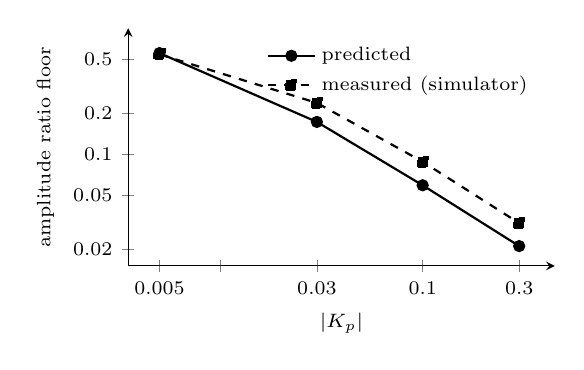
\begin{tikzpicture}
        \begin{axis}[width=7.0cm, height=4.6cm,
                     xmode=log, ymode=log,
                     xlabel={$|K_p|$}, ylabel={amplitude ratio floor},
                     xtick={0.005,0.01,0.03,0.1,0.3},
                     xticklabels={0.005,,0.03,0.1,0.3},
                     ytick={0.02,0.05,0.1,0.2,0.5},
                     yticklabels={0.02,0.05,0.1,0.2,0.5},
                     xmin=0.0035, xmax=0.45, ymin=0.015, ymax=0.85,
                     axis lines=left, legend pos=north east,
                     legend style={draw=none, fill=none},
                     legend cell align=left, mark size=1.8pt]
          \addplot[thick, mark=*] coordinates
            {(0.005,0.557) (0.030,0.173) (0.100,0.059) (0.300,0.021)};
          \addlegendentry{predicted}
          \addplot[thick, dashed, mark=square*] coordinates
            {(0.005,0.545) (0.030,0.239) (0.100,0.088) (0.300,0.031)};
          \addlegendentry{measured (simulator)}
        \end{axis}
      \end{tikzpicture}
    \end{column}
    \begin{column}{0.46\textwidth}
      \footnotesize
      The ratio settles at \textbf{0.23}, and that is the \emph{steady state of
      a continuously forced oscillator}, not a failure to converge. Remove the
      drive mid-run and it decays with $\tau = 3.4$\,s damped against 15.9\,s
      gain-off (predicted 2.76 / 15.92).

      \vspace{2mm}
      The floor tracks $\dfrac{\text{intrinsic}}{\text{intrinsic} +
      \text{added}}$ damping, so it falls monotonically with gain.

      \vspace{2mm}
      \textbf{The floor falls with gain, and gain is capped at
      $|K_p| = 0.035$ by the instability bound.} Those two facts are the vice
      the project sits in.

      \vspace{2mm}
      The residual \textbf{0.0089\,V} is the actuator's 0.5\,mV deadband and
      10\,ms throttle, \emph{not} sensing: $0.0089 / 0.0087 / 0.0094$\,V at
      $20 / 5 / 0$\,mV of injected sensor noise. Fixing it moves 0.009 to 0.009
      while you sit at 0.23.
    \end{column}
  \end{columns}
\end{frame}
\note{One physics slide before closing, because it explains where the project is
stuck.

The amplitude ratio does not go to zero. It settles around 0.23, and that is not
a failure to converge, it is the steady state of a continuously forced
oscillator. The proof: remove the drive mid-run and it decays with a 3.4 second
time constant damped, against 15.9 with the gain off, both close to prediction.

The floor tracks the ratio of intrinsic damping to intrinsic plus added damping.
So the floor falls with gain, monotonically, confirmed from 0.005 to 0.300.

Which puts the project in a vice. The only way below 0.23 with this control law
is more gain, and gain is capped by a limit at minus 0.04 that nobody has ever
characterised. That is why characterising it is ranked where it is.

And a nice negative result: the residual of 0.0089 volts is not sensor noise.
Inject twenty, five or zero millivolts and it barely moves. It is the actuator's
half-millivolt deadband and ten-millisecond throttle. Fixing that would move you
from 0.009 to 0.009 while you are sitting at 0.23.}

% ================================================================ 54
\begin{frame}{What the simulator can and cannot tell you}
  \begin{columns}[T]
    \begin{column}{0.48\textwidth}
      \footnotesize
      \textbf{It runs the \emph{real} controller.} Every version is imported and
      stepped, not reimplemented. Only \texttt{serial} and
      \texttt{DACController} are stubbed.

      \vspace{2mm}
      \textbf{\texttt{SIM\_CHANNELS = (4, 8)}}, against a \emph{measured}
      eight-OSEM body. Four- and eight-channel controllers are both
      simulated. Only \texttt{osem.\texttt{sysid}.py} and \texttt{osem.the unwritten build.py} are skipped,
      both by \texttt{KIND}.

      \vspace{2mm}
      The plant is a linear second-order oscillator per mode with \textbf{exactly
      one nonlinearity}: the ADC, which offsets each channel to its resting
      count, rounds, and hard-clips at 0/1023. That is why clipping emerges on
      its own, with the bench's asymmetry.
    \end{column}
    \begin{column}{0.5\textwidth}
      \footnotesize
      \textbf{What it cannot tell you:}
      \begin{itemize}\setlength{\itemsep}{2pt}
        \item \textbf{A safe gain.} More negative $K_p$ is monotonically more
              damping all the way to $-0.6$. The ADC model reproduces
              \emph{clipping}, not instability.
        \item \textbf{A wrong coil map.} It round-trips its held-voltage dict
              through whatever map the controller declares. \textbf{Only the
              bench catches one.}
        \item \textbf{A torn serial frame.} The transport is stubbed, so
              defect 7 could not have been found here.
      \end{itemize}

      \vspace{2mm}
      \textbf{\texttt{make check}: 220 passed, 11 failed} in 925\,s.
      \texttt{sample-guard}, \texttt{decimate} and all five
      \texttt{persist-baseline} assertions pass. The 11 failures are in
      \texttt{warm-restart} / baseline-reuse and are \emph{not yet
      attributed}: only 2 of the 11 were ever read.
    \end{column}
  \end{columns}
\end{frame}
\note{A slide about epistemics, because it is what keeps the numbers in this deck
trustworthy.

The strength is that it runs the real controller: every version is imported and
stepped, not reimplemented, with only the serial module and the DAC controller
stubbed. So a behavioural result here is a result about the code that runs on the
bench.

The one nonlinearity is the ADC, which is why clipping emerges on its own in
simulation with the bench's actual asymmetry.

The blind spots. It cannot tell you a safe gain, because the plant is linear and
damping increases monotonically to minus 0.6. It cannot catch a wrong coil map,
because it round-trips its held-voltage dictionary through whatever map the
controller declares. And it could not have found the torn serial frame, because
the transport is exactly the thing that is stubbed.

Finally, be honest about the suite as it stands: 220 passed and 11 failed. The
fixes delta introduced all pass. The failures are in warm-restart and baseline
reuse, and they are not yet attributed, because the run that produced them was
captured through tail minus 25, so only two of the eleven were ever read. Re-run
it and read all of it before trusting any of them.}

% ================================================================ 55
\begin{frame}{Still open, in the order I would do them}
  \footnotesize
  \begin{enumerate}\setlength{\itemsep}{1.5pt}
    \item \alert{\textbf{\texttt{LOCKED} is never announced.}} a5 vetoes the
          quorum at ratio 1.26--2.53 against 0.35 while nothing drives it.
          \textbf{One line}, and it is the deliverable.
    \item \textbf{The bias sweep.} Step one channel $0.10 \to 0.40$\,V at zero
          gain, log resting counts. Settles whether the 601/630/687/682 offset
          is electromagnetic or mechanical. \textbf{No code.}
    \item \textbf{Confirm \texttt{delta}'s gain cut on the bench.} Peak demand
          $0.2998 \to 0.2001$\,V, dissipative share $43\% \to 88\%$.
    \item \textbf{Cut \texttt{LOCK\_SUSTAIN\_S} $= 5.0$}, on its own: five of
          the ten-second budget confirming a lock that already happened.
    \item \textbf{Gate fault re-engagement on amplitude}, not a fixed 5\,s,
          which is 35 of \texttt{delta}'s 35.2 fault-seconds.
    \item \textbf{Kalman velocity estimator}, unblocked: $f$ to 0.0001\,Hz,
          $\tau > 138$\,s so $Q$ stops mattering, measurement noise measured.
    \item \textbf{Read all 11 \texttt{make check} failures.} Only 2 were seen.
    \item \textbf{a4, a6, a7.} Connected, near mid-scale, $\sim$1/100 the
          in-band gain of a0--a3. Cause not established.
  \end{enumerate}

  \vspace{1.5mm}
  \centering
  \emph{Learn the model, the estimator and the anomaly detector; keep the
  control law and the interlocks classical and certifiable.}
\end{frame}
\note{Eight things, in the order I would do them.

One, and it is first because it is the stated deliverable: the rig has not
announced LOCKED since 2026-08-04, and the cause is a quorum bug worth one line.

Two, the bias sweep. It is the highest-value experiment available because it may
solve the clipping problem with no hardware work at all, and it needs no code:
two commands and a log.

Three, confirm delta's gain cut on the bench. That is the arithmetic that takes
peak demand back inside the actuator window.

Four and five are the lock-time budget: five seconds confirming a lock that
already happened, and five seconds of mandatory hold after every fault, which is
now the entire fault cost.

Six, the Kalman estimator, which is newly unblocked because the frequencies are
known to a tenth of a millihertz and the intrinsic decay is long enough that Q
stops mattering on control timescales.

Seven is bookkeeping with teeth: eleven suite failures exist and only two of them
have ever been read.

Eight is the honest one. a4, a6 and a7 are connected, sit near mid-scale, and carry
about a hundredth of the in-band gain of the working four. We do not know why, and
the deck used to claim we did.

And the closing principle, which I think is right for anything that can destroy a
suspended mirror: learn the model, the estimator and the anomaly detector, and
keep the control law and the interlocks classical and certifiable.}

% ================================================================ 56
\begin{frame}{The ladder, end to end}
  \centering
  {\scriptsize\setlength{\tabcolsep}{2.2pt}
  \begin{tabular}{@{}llllccl@{}}
    \toprule
     & channels & I/D & what it added & ch0 ratio & lock & bench \\
    \midrule
    \texttt{zero}    & ch0 only  & zeroed & \emph{the baseline} & 0.188 & 12.1\,s & 2026-07-15 (scope) \\
    the early four-channel build    & all four  & zeroed & all four channels on & 0.025 & 10.7\,s & 2026-08-03 \\
    the early four-channel build    & all four  & live   & real $K_i$, $K_d$ & 0.028 & 10.5\,s & 2026-08-03 \\
    \texttt{alpha}    & all four  & live   & \textbf{all 3 defects fixed} & 0.029 & 10.6\,s & \textbf{validated} \\
    \addlinespace
    \texttt{alpha}    & all four  & live & \texttt{auto-disable} & 0.029 & 10.6\,s & 2026-08-04 \\
    the build before \texttt{beta}    & all four  & live & \texttt{fast-refault} & 0.029 & 10.6\,s & 2026-08-04 \\
    the eight-OSEM step  & \emph{all eight} & live & eight-OSEM build & n/a &
      \emph{10 faults} & 08-04, no lock \\
    \texttt{sysid}    & \multicolumn{5}{l}{\emph{bench tool}: stepped-sine actuation matrix, closes no loop} & 08-04 \\
    the bias-trim branch    & all four  & live & \texttt{bias-trim} & 0.029 & 10.6\,s & \textbf{validated} \\
    the build before \texttt{beta}    & all four  & live & \texttt{fast-calib}, \texttt{warm-restart} & 0.029 & 10.5\,s & 2026-08-04 \\
    \textbf{\texttt{beta}} & all four & live & \textbf{\texttt{runaway-trend}} & 0.029 & 10.5\,s & \textbf{83.1\% 08-04} \\
    the eight-channel step   & 5 of 8 & live & \texttt{soft-saturation}, \texttt{baseline-floor}
      & n/a & n/a & 74.1\% 08-06 \\
    the 500000-baud step   & \emph{all eight} & live & \texttt{sat-window}, \texttt{fast-transport}
      & n/a & n/a & 42.3\% 08-06 \\
    \textbf{\texttt{delta}} & \emph{all eight} & \textbf{cut} &
      \textbf{\texttt{sample-guard}, \texttt{decimate}, LAG} & n/a & n/a &
      \textbf{77.5\% 08-06} \\
    the unwritten build   & \multicolumn{5}{l}{\emph{skeleton}: refuses to run} & n/a \\
    \bottomrule
  \end{tabular}}

  \vspace{1mm}
  {\scriptsize\sloppy
  Ratios and lock times are \textbf{simulator} numbers; the percentages are
  \textbf{time-weighted \texttt{DAMPING}} on the bench. \texttt{beta}'s 83.1\% and
  \texttt{delta}'s 77.5\% ran different kick schedules and are not comparable.
  \textbf{The control law did not change from the early four-channel build to the 500000-baud step}: everything between is
  the supervisor around it. \texttt{make check}: \textbf{220 passed, 11
  failed}.}
\end{frame}
\note{The whole ladder on one slide.

The single most important thing to read off it is the ch0 ratio column: 0.029
from alpha all the way to beta. The control law did not change between the early four-channel build and the 500000-baud step.
Every version in between is the supervisor around it: when the loop is allowed to
be closed, what counts as a fault, how a fault is recovered from, and how the
baseline everything scales off is measured. delta is the first version since alpha to
move a gain, and it moved them because of an arithmetic budget rather than a
retune.

Read the last four rows carefully and read the caveat under the table. beta's 83.1
percent and delta's 77.5 are not comparable: beta's three kicks were scripted and
delta's five were by hand. The comparison that is controlled is the 500000-baud step at 42.3 against
delta at 77.5, same session, same schedule, and delta against itself across the lag
change.

Four rows read validated: alpha, the bias-trim branch, beta and the eight-channel step. On four channels the one to reach
for is still beta. On eight channels it is delta, and delta is the one to develop
against.

And the row at the bottom is the unwritten build, which is not a version. It is a skeleton that
refuses to run, and until yesterday it did not refuse.}

\end{document}
